\documentclass[orivec]{llncs}
\usepackage{graphicx}
\usepackage{amsmath}			% for "cases"
\usepackage{amsfonts}		% for frakur fonts
\usepackage{mathrsfs}		% for curly "E" error symbol
\usepackage{float}
\usepackage[most]{tcolorbox}	% for wrapping example in color box
% \usepackage{wrapfig}			% wrap figure beside text, used in example
\usepackage{tikz-cd}			% commutative diagrams
\usepackage{tikz}
\usepackage{amssymb}			% for \multimap \updownarrow \bigstar \varnothing
\usepackage{sectsty}			% change section color
% \usepackage{turnstile}		% longer turnstiles
\usepackage{wasysym}			% smileys
\usepackage[normalem]{ulem}	% underline with line breaks: /uline
\usepackage{hyperref}		% refs, links become clickable
\usepackage[]{algorithm2e}	% algorithms

\usepackage{geometry}		% change paper size
\geometry{
  a4paper,         % or letterpaper
  textwidth=18cm,  % llncs has 12.2cm
  textheight=27cm, % llncs has 19.3cm
  heightrounded,   % integer number of lines
  hratio=1:1,      % horizontally centered
  vratio=2:3,      % not vertically centered
}
\usepackage[fontsize=13pt]{scrextend}

% *************** Delete when not using Chinese or colors **********************
% \usepackage{xeCJK}
% \setCJKmainfont[BoldFont=SimHei,ItalicFont=KaiTi]{SimSun}

\usepackage{color}
\definecolor{cerulean}{RGB}{100,100,200}
\definecolor{darkgreen}{RGB}{10,130,10}
%\newcommand{\emp}[1]{\textbf{\textcolor{Cerulean}{#1}}}
\newcommand{\emp}[1]{\textbf{#1}}
\definecolor{grey}{rgb}{0.9,0.9,0.9}  % grey

% \chapterfont{\color{blue}}		% sets colour of chapters
\sectionfont{\color{blue}} 
\subsectionfont{\color{blue}} 
\subsubsectionfont{\color{blue}} 
\setcounter{secnumdepth}{3}		% use numbers in subsubsections
% \renewcommand\thesection{}		% hide section numbers (has bad indent effect)

\let\emptyset\varnothing			% more beautiful empty set symbol
\newcommand{\vect}[1]{\boldsymbol{#1}}
\newcommand*\sigmoid{\vcenter{\hbox{
\includegraphics{sigmoid.png}}}}
\newcommand*\KB{\vcenter{\hbox{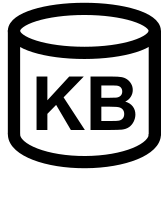
\includegraphics{KB-symbol.png}}}}
\newcommand*\NN{\vcenter{\hbox{\includegraphics{NN-symbol.png}}}}
\newcommand*\invsigmoid{\vcenter{\hbox{\includegraphics{inverse-sigmoid.png}}}}
\newcommand{\invW}{\, \rotatebox[origin=c]{90}{W}}
\newcommand{\invw}{\, \rotatebox[origin=c]{90}{w}}
\newcommand*\rectifier{\vcenter{\hbox{\includegraphics{rectifier.png}}}}
\newcommand{\dashh}{\textemdash~}
\newcommand{\tab}{\hspace*{1cm}}

\newcommand{\tikzmark}[1]{\tikz[overlay,remember picture] \node (#1) {};}

\let\labelitemi\labelitemii

\renewcommand{\thefootnote}{\fnsymbol{footnote}}
\interfootnotelinepenalty=10000

% ***** Boxed variables inside math equations
% \newcommand*{\boxedcolor}{black}
\makeatletter
% \renewcommand{\boxed}[1]{\textcolor{\boxedcolor}{%
% \fbox{\normalcolor\m@th$\displaystyle#1$}}}
% \setlength{\fboxsep}{1pt}
\renewcommand{\boxed}[1]{\fbox{\m@th$\displaystyle\scalebox{0.9}{#1}$} \,}
\makeatother

\overfullrule=0mm

\newsavebox{\MyName}
\savebox{\MyName}{
\includegraphics[scale=0.6]{YKY.png}}

\title{What are neural networks?\\
{\normalsize (requires only high-school maths)}}
\titlerunning{What are neural networks?}
\author{\usebox{\MyName} (King-Yin Yan)
% \\ \footnotesize{General.Intelligence@Gmail.com}
}
\institute{General.Intelligence@Gmail.com}

\begin{document}

\maketitle
\setlength{\parindent}{0em}
% \setlength{\parskip}{2.8ex plus0.8ex minus0.8ex}
\setlength{\parskip}{2.8ex}

%\begin{abstract}
%\end{abstract}

The 3 main approaches in artificial intelligence are:
\begin{itemize}
 \item logic
 \item neural networks
 \item evolution
\end{itemize}
Neural networks is a special kind of \textbf{statistical learning}, that operates on ``points'' in a vector space.

Deep learning is the hottest technique in current AI research.  ``Deep'' simply means ``many layers of neural networks''.

\section*{Biological neurons}

Let's refresh some high-school biology {\Large \smiley}

This is a biological neuron:
\begin{equation}
\vcenter{\hbox{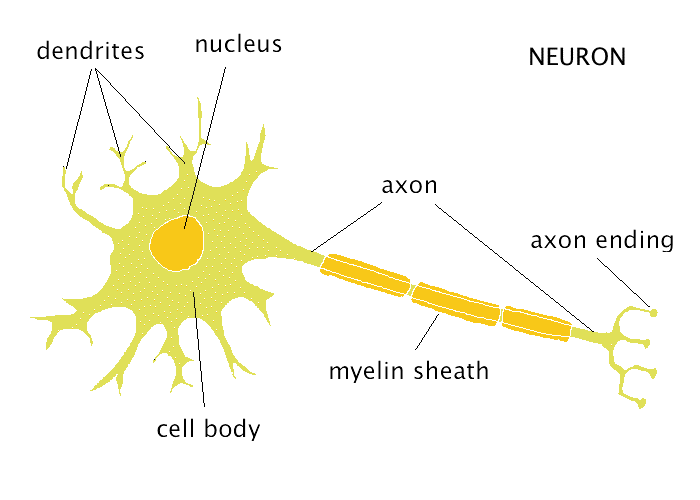
\includegraphics[scale=0.4]{neuron.png}}}
\end{equation}
Dendrites \textbf{collect} electrical signals;  When the \textbf{total} of these signals exceed a certain \textbf{threshold}, the neuron \textbf{fires} an electric impulse, sending to another neuron via the \textbf{axon}:

\begin{equation}
\vcenter{\hbox{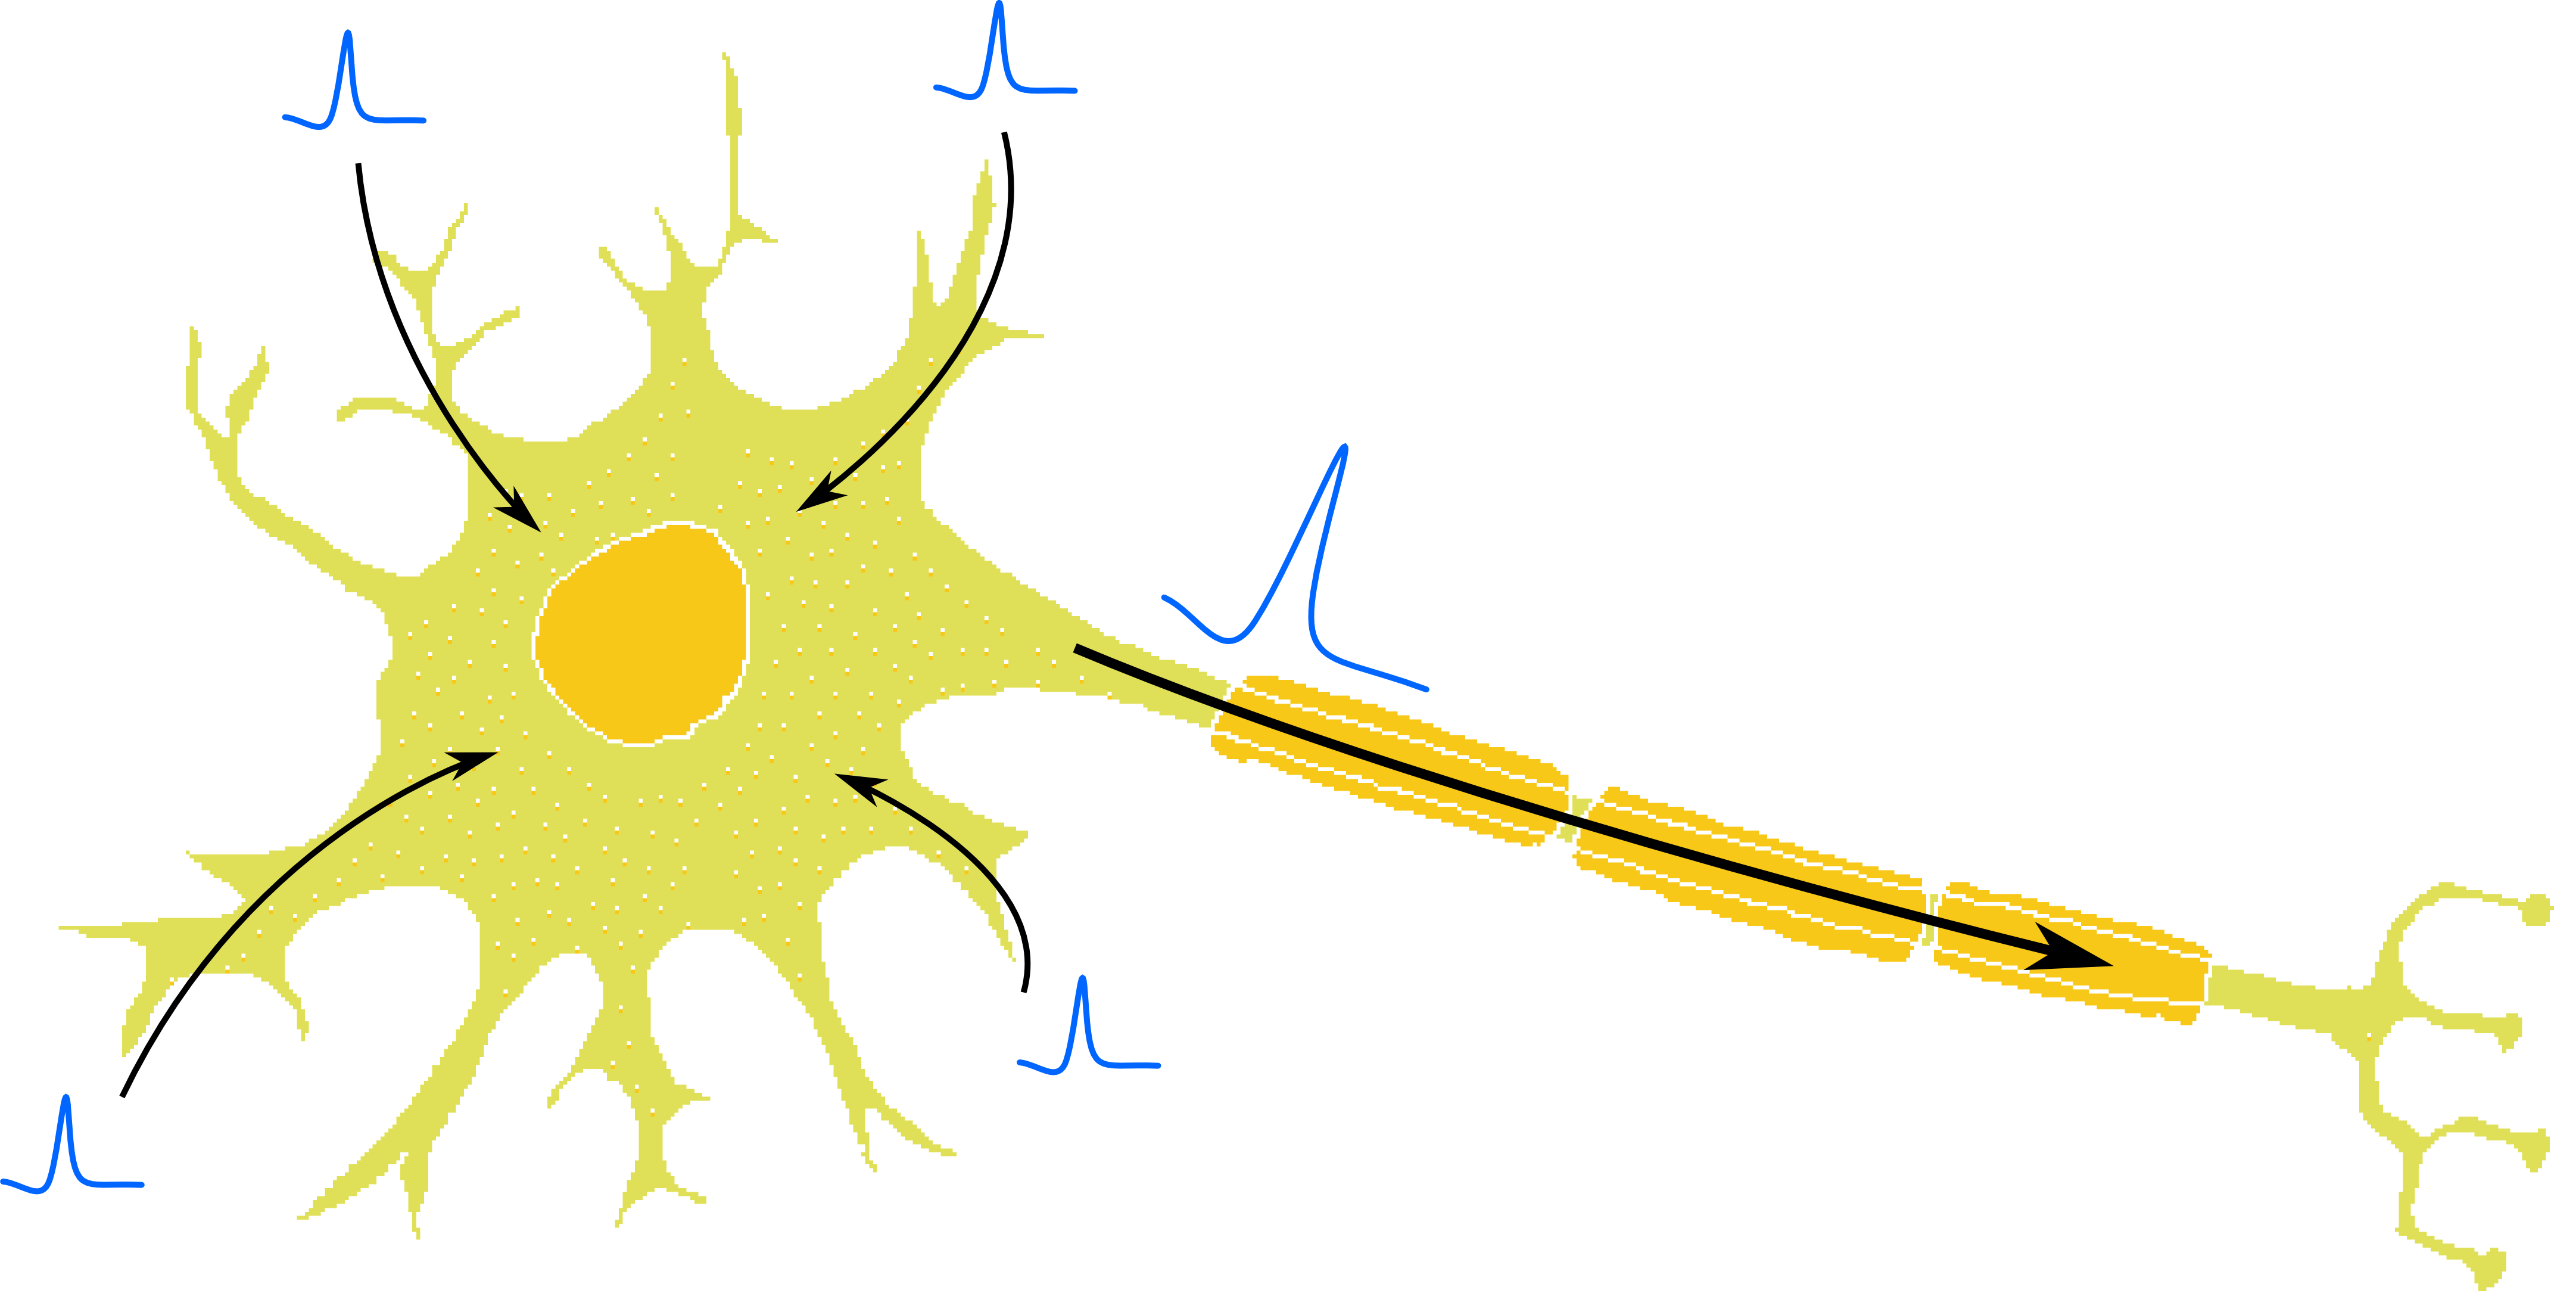
\includegraphics[scale=0.5]{neuron-firing.png}}}
\end{equation}
Mathematically, this can be greatly simplified to such a \textbf{model}:
\begin{equation}
\vcenter{\hbox{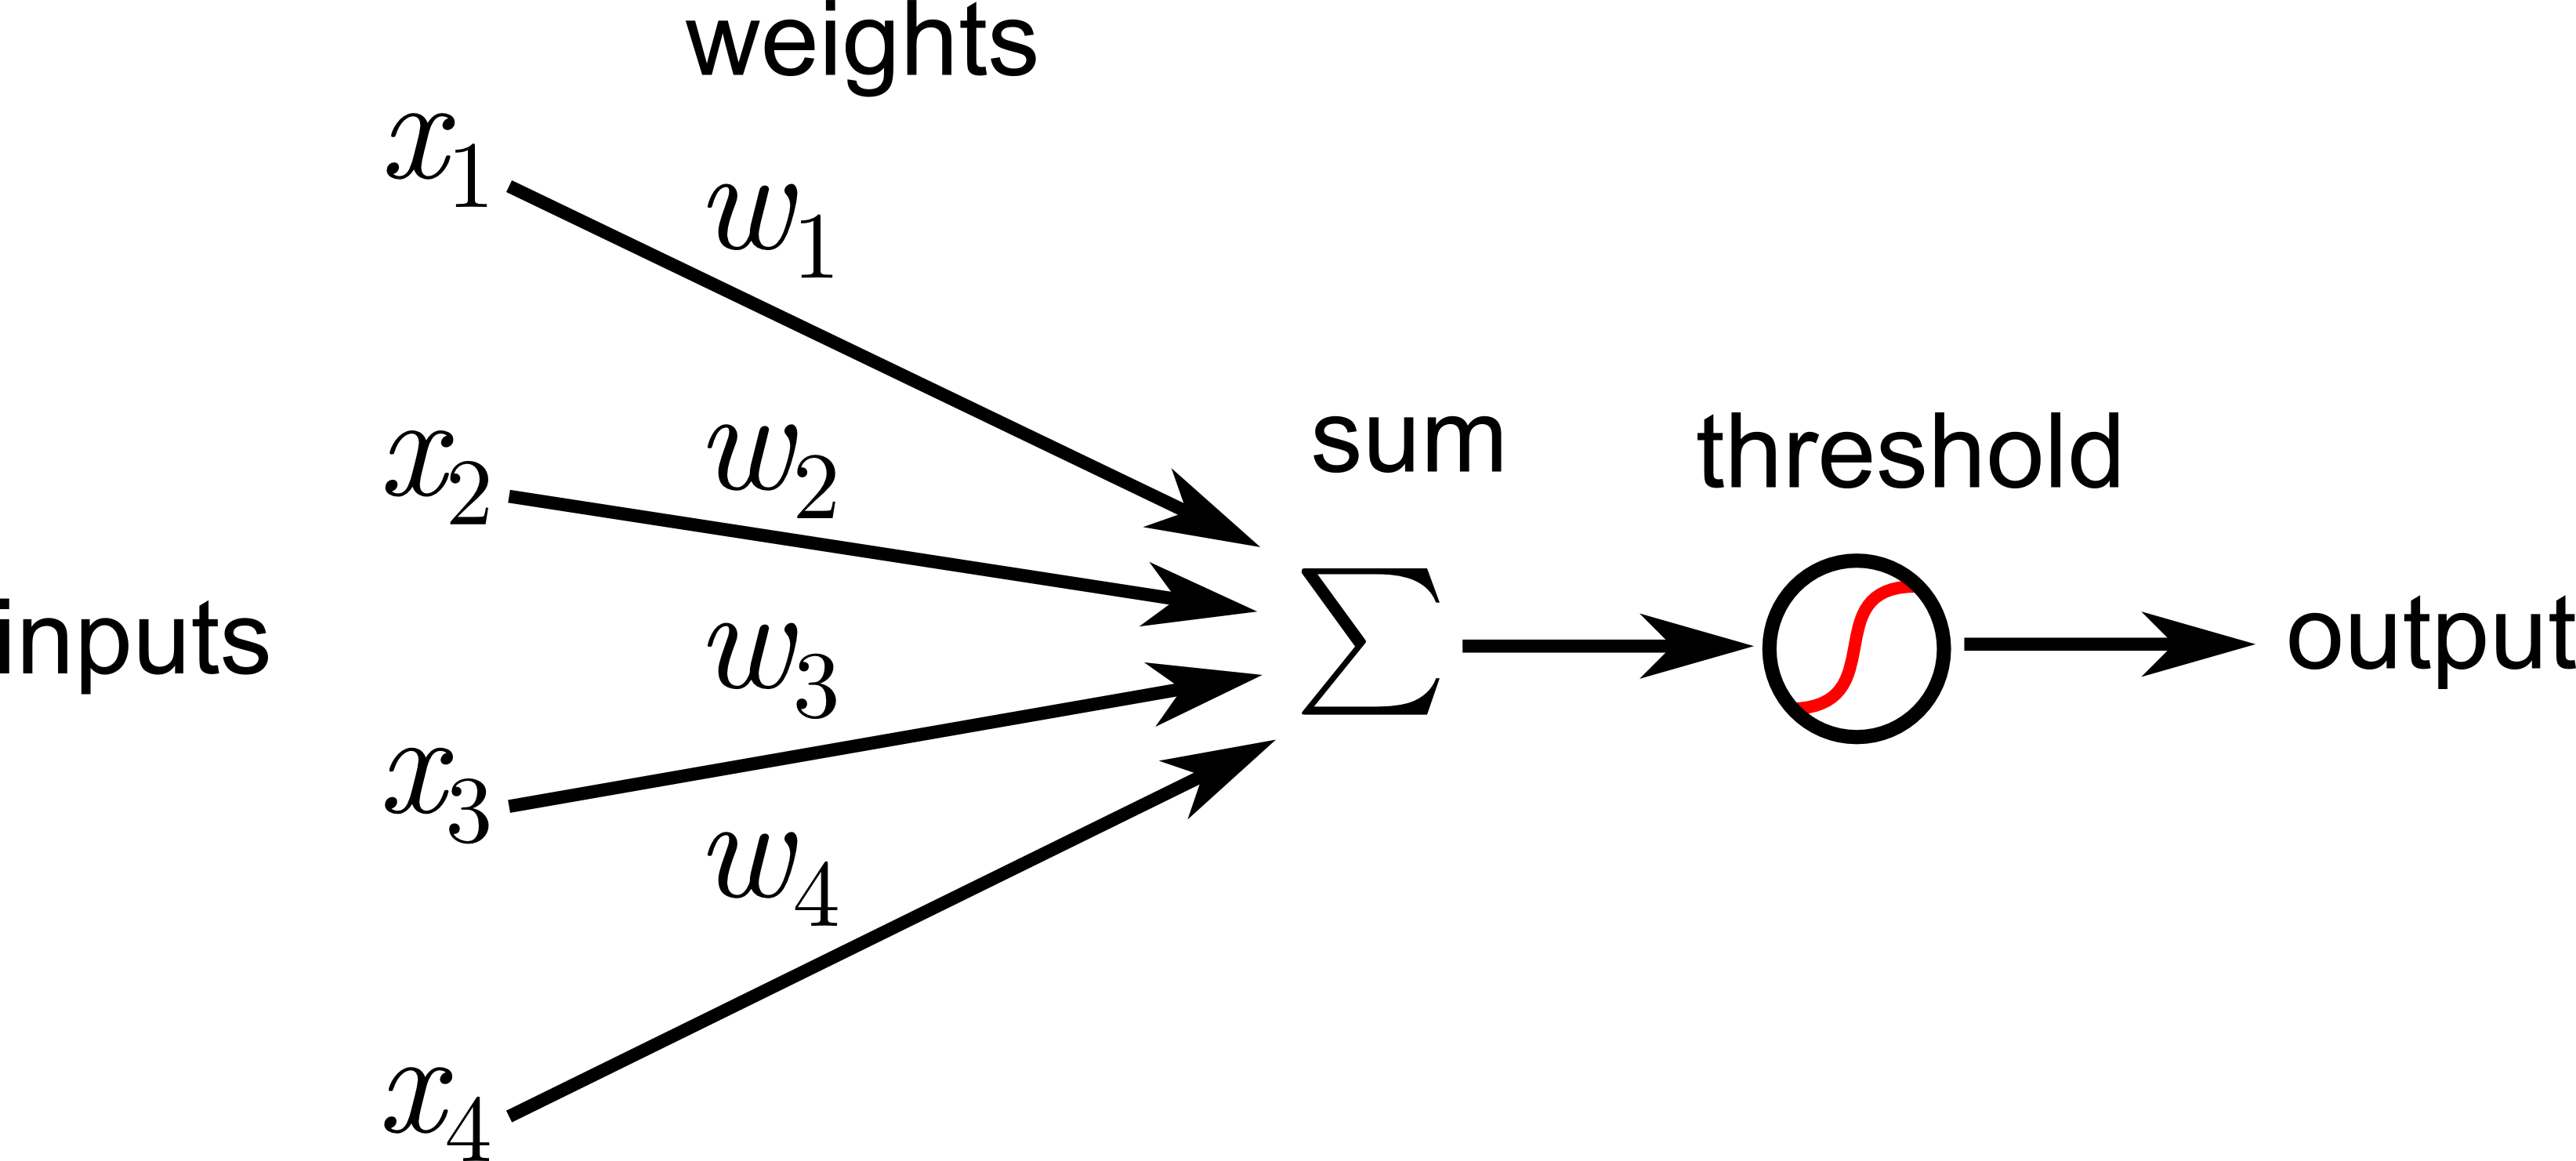
\includegraphics[scale=0.75]{neuron-model.png}}}
\end{equation}
That means:  each input value is \textbf{weighted} and then summed together, and then passes through a $\sigmoid$ function for output.

In formula:
\begin{equation}
\boxed{output} \; y = \sigmoid \; [ \; \sum_i (w_i \; x_i) \; ]
\end{equation}
where $\sigmoid$ = sigmoid function, is defined by:
\begin{equation}
\sigmoid (x) = \frac{1}{1 + e^{-x}}
\end{equation}
Its shape is like this:
\begin{equation}
\vcenter{\hbox{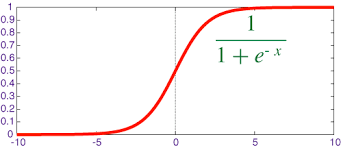
\includegraphics[scale=0.55]{sigmoid-graph.png}}}
\end{equation}
On the left it is 0 = nothing (no signals), on the right it is 1 = ``yes''.

These functions can all play the role of the ``threshold'':
\begin{equation}
\vcenter{\hbox{\includegraphics[scale=0.5]{../AGI-17/activation-functions.png}}}
\end{equation}

\begin{tcolorbox}[breakable, enhanced]
\textbf{Fun fact \#1}\\

The surface of the neuron is covered with sodium-potassium (Na$^+$/K$^+$) channels, that use ATP (adenosine triphosphate, the energy source in the cell) to ``pump'' ions into the cell with a 3 Na$^+$ : 2 K$^+$ ratio, creating a voltage difference.   When the voltage exceeds the threshold, certain ion channels open, the built-up voltage is released to create an ``action potential''.  This phenomenon can be described using differential equations, that is the famous \textbf{Hodgkin-Huxley} equation, and its simplified version, the \textbf{FitzHugh-Nagumo} equation.\\

A very special feature about the action potential is that it is ``\textbf{all-or-nothing}'', ie, if the input is below threshold, the output signal would be flat (zero).  Why is it like this?  That is because the human brain evolved from primitive \textbf{multi-cellular} organisms (like the jellyfish) whose cells gradually learned to use electric signals to communicate.  They operated in an environment like a pool of water, in which there is a lot of \textbf{noise}.  Even now the human brain is like a pool of liquid, and the body is in constant motion, resulting in \textbf{heat noise}.  In order to operate within such noise, there must be a mechanism to \textbf{suppress} the noise;  This is the reason for all-or-nothing.  That is to say, human consciousness has \textbf{finite} information content, similar to a digital computer, and is not mysterious.
\end{tcolorbox}

\begin{tcolorbox}[breakable, enhanced]
\textbf{Fun fact \#2} \\

The neuron's \textbf{cell membrane} is a \textbf{lipid bi-layer}, made up of fats and cholesterol.  The function of cholesterol is to make the membrane structurally stable, therefore every cell needs cholesterol.  The ``wires'' in the brain are all made of cell membranes, so the brain is basically made up of fats and cholesterol.  In particular, the pig's brain which is a kind of Chinese food, has the highest cholesterol content of all foods, many times more than eggs! \\

The \textbf{myelin sheath}, unique to vertebrates, is like the plastic insulation of electric wires, whose effect is to speed up electrical transmission.  The octopus is an invertebrate, that's why it needs a big head to achieve the same level intelligence as vertebrate animals of comparable brain size.
\end{tcolorbox}

\begin{tcolorbox}[breakable, enhanced]
\textbf{Fun fact \#3} \\

When the nerve signal reaches the \textbf{synapse}, it no longer uses electrical transmission, but switches to chemical transmission with \textbf{neuro-transmitter} molecules.  There are many types of neuro-transmitters, such as \textbf{serotonin} and \textbf{dopamine}, often mentioned in anti-depression drugs.  But the most common neuro-transmitter is \textbf{glutamate}, the main signaling molecule for the nervous systems of all animals.  Plants lack a nervous system, therefore glutamate is not found in plants.  Humans like to eat meat, so we evolved a taste for meat, especially the taste for glutamate.  A Japanese scientist discovered a substance in sea-weed, which when added to food mimics the taste of meat.  Actually this substance is just glutamate, or MSG (mono-sodium glutamate).  So MSG is not harmful to humans, it's just that we may not get a balanced nutrition if we eat MSG often instead of real meat.
\end{tcolorbox}

\section*{1 neuron -- geometric interpretation}

As I explained in other tutorials, the goal of \textbf{machine learning} is usually to \textbf{classify} certain ``points'' in a space:
\begin{equation}
\vcenter{\hbox{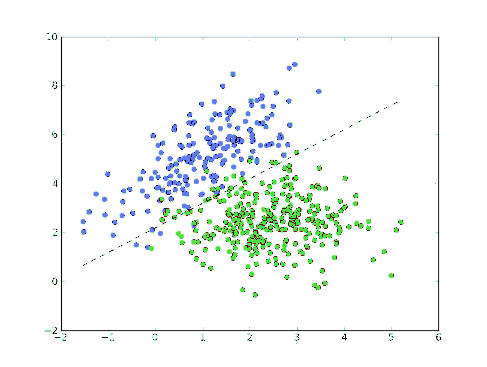
\includegraphics[scale=0.6]{ML-example.png}}}
\end{equation}

For example, in \textbf{machine vision}, a picture can have millions of \textbf{pixels}, each pixel being a dimension, its \textbf{color} is the \textbf{coordinate value} on this dimension.  The entire space is the space of \textbf{all images}, with each \textbf{point} representing an image.  The dimensionality of such spaces is very high (the dimension is the number of pixels per image).  We often use 2 or 3 dimensions for explaining things, but the reader should use their imagination for higher dimensions.

We know from high-school maths, the equation for a \textbf{straight line} is:
\begin{eqnarray}
& \mbox{\footnotesize \color{red}{constants}} \tikzmark{constants} \nonumber \\
\nonumber \\
& {\color{red}{a}} \tikzmark{constA} x \tikzmark{varX} + {\color{red}{b}} \tikzmark{constB} y \tikzmark{varY} + {\color{red}{c}} \tikzmark{constC} = 0 \\
\nonumber \\
& \mbox{\footnotesize variables} \tikzmark{variables} \nonumber
\begin{tikzpicture}[overlay,remember picture]
  \draw[red] (constants.center) +(-30pt,-4pt) -- ([shift={(-3pt,8pt)}]constA.center);
  \draw[red] (constants.center) +(-20pt,-4pt) -- ([shift={(-1pt,10pt)}]constB.center);
  \draw[red] (constants.center) +(-10pt,-4pt) -- ([shift={(-1pt,8pt)}]constC.center);
  \draw (variables.center) +(-29pt,8pt) -- ([shift={(-4pt,-2pt)}]varX.center);
  \draw (variables.center) +(-15pt,8pt) -- ([shift={(-4pt,-4pt)}]varY.center);
\end{tikzpicture}
\end{eqnarray}

Its \textbf{geometric interpretation} is like this:
\begin{equation}
\vcenter{\hbox{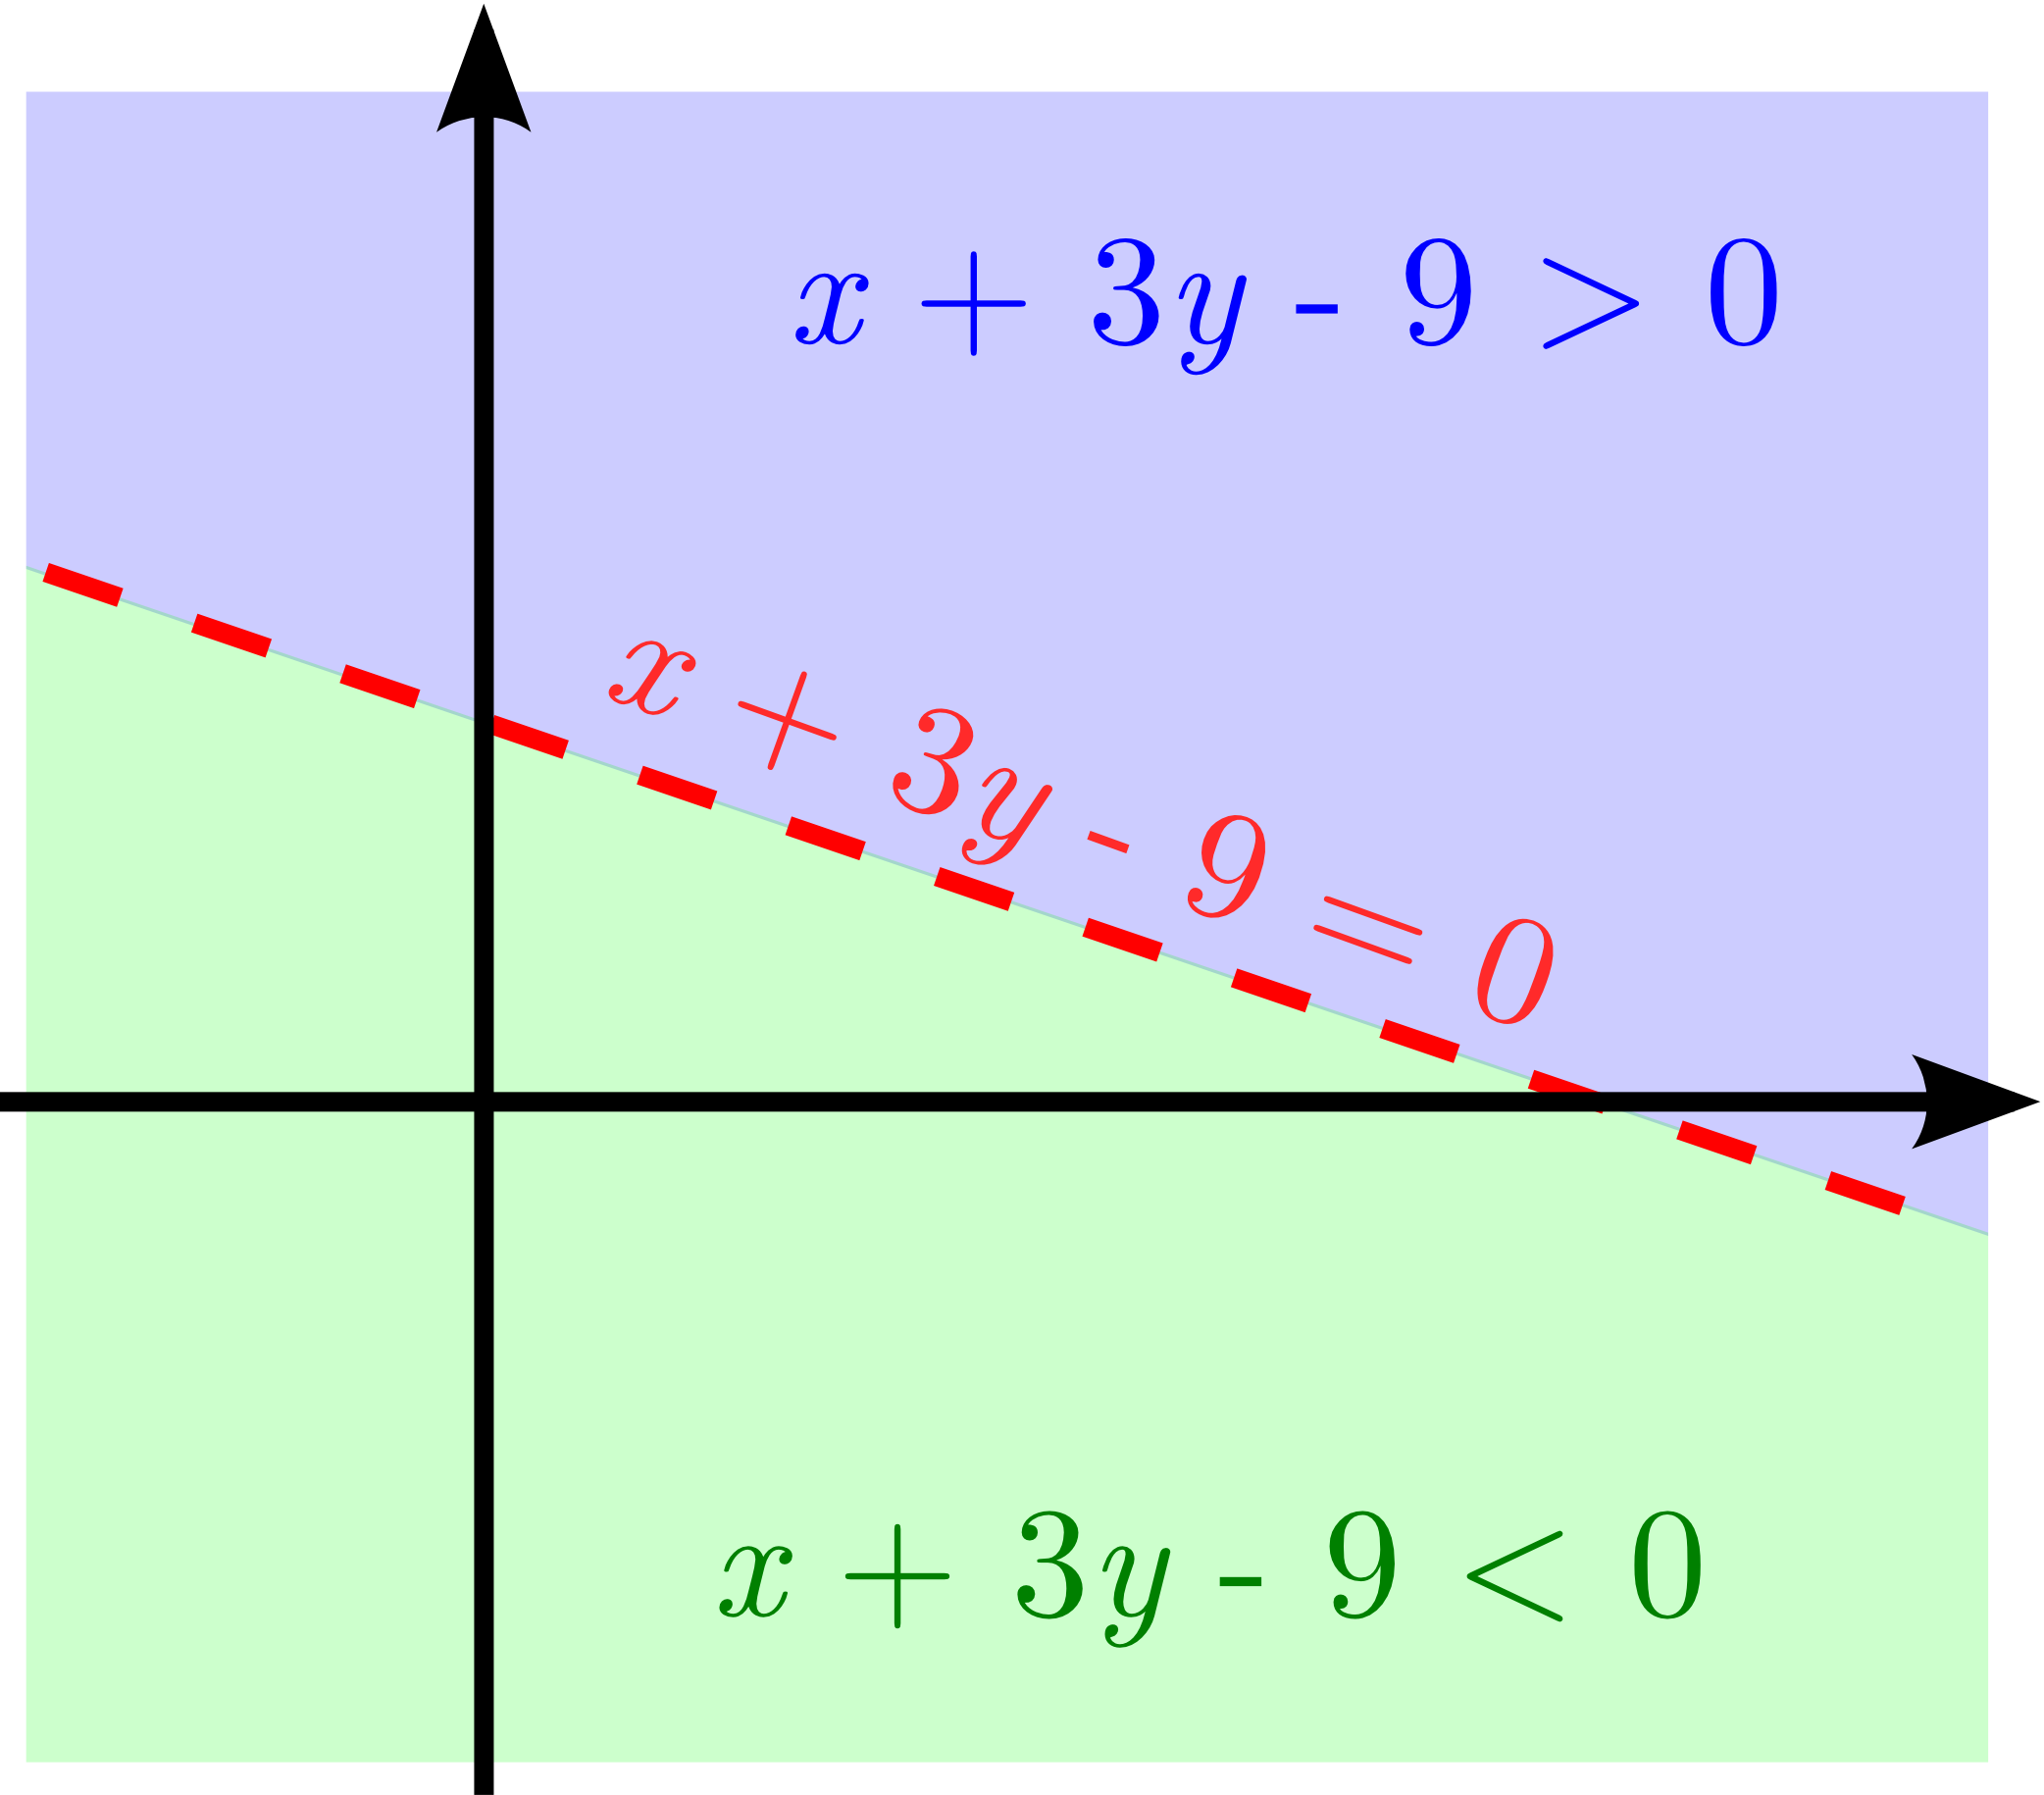
\includegraphics[scale=0.75]{linear-inequality.png}}}
\end{equation}
For points on the line, the equation is $= 0$.  The line \textbf{cuts} the space into 2 halves:  one side is $> 0$, the other $< 0$.

Generalizing to 3-dimensions, we have the equation for a \textbf{plane}:
\begin{equation}
{\color{red}{a}}x + {\color{red}{b}}y + {\color{red}{c}}z + {\color{red}{d}} = 0
\end{equation}
It also \textbf{cuts} the space into 2 halves, one side $> 0$, the other $< 0$:
\begin{equation}
\vcenter{\hbox{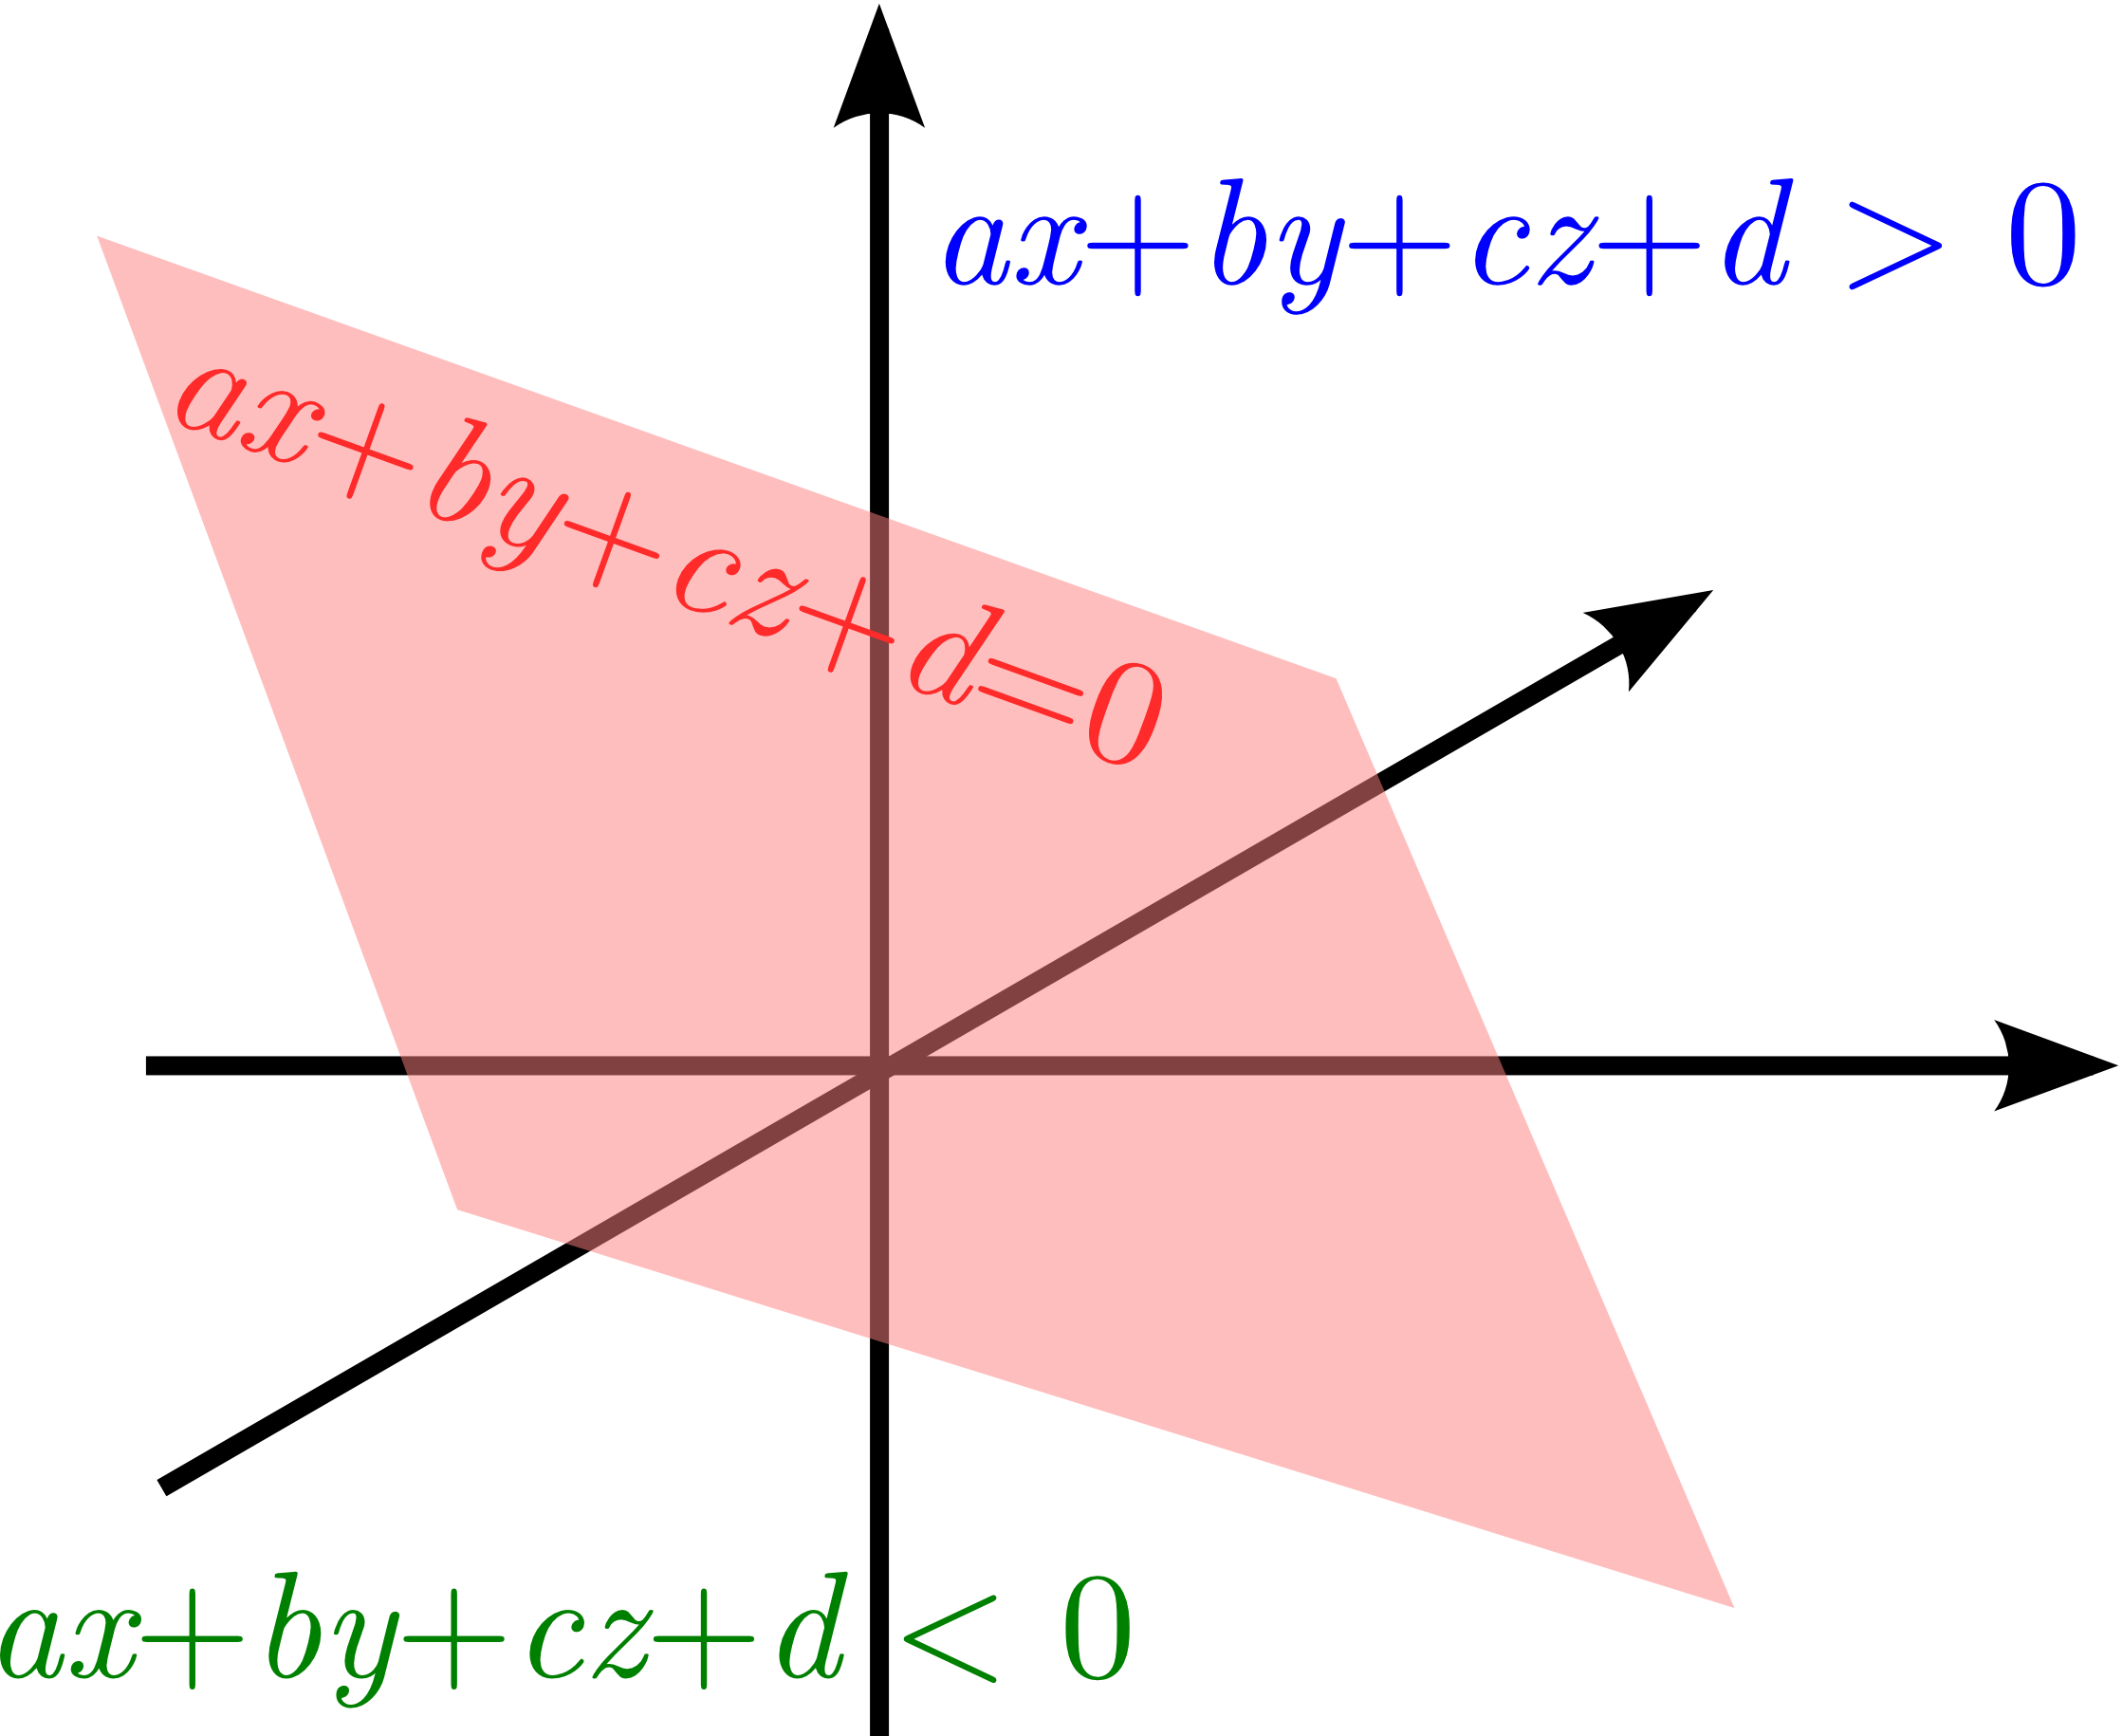
\includegraphics[scale=0.75]{linear-inequality-2.png}}}
\end{equation}

For arbitrary $n$-dimensions, with each point denoted as $\vect{x} = (x_1, x_2, ..., x_n)$, a \textbf{hyperplane} cuts the space into 2 halves, its equation is:
\begin{equation}
{\color{red}{a_1}}x_1 + {\color{red}{a_2}}x_2 + .... + {\color{red}{a_n}}x_n + {\color{red}{a_0}} = 0
\label{eqn:general-linear}
\end{equation}

\begin{tcolorbox}[breakable, enhanced]
Note:  What is the dimension of a hyper-plane?  In 2-D space, it is a line (1-D), in 3-D space, it is a plane (2-D);  In general, in $n$-D space a hyper-plane is an $(n - 1)$-dimension object, $(n-1)$ is also called \textbf{co-dimension 1}, meaning that the ambient space is of dimension $n$, and equation (\ref{eqn:general-linear}) reduces the \textbf{degrees of freedom} by 1, so the object \textbf{constrained} by this equation has $n - 1$ degrees of freedom.
\end{tcolorbox}

Now we can see some resemblance between the hyper-plane and the neuron, as the neuron is a \textbf{linear combination} before passing to the $\sigmoid$:
\begin{eqnarray}
& \mbox{\footnotesize \color{red}{linear combination}} \nonumber \\
\boxed{output} \; y = \sigmoid & [ \; \overbrace{\sum_i (w_i \; x_i)} \; ]
\end{eqnarray}
That is to say:  \uline{Each neuron forms a hyper-plane, that cuts the space into 2 halves}.

What if $\sigmoid$ is applied?  Without $\sigmoid$, the 2 halves are $> 0$ and $< 0$;  Now if we see colors as ``intensity'', the intensity changes gradually:  (the figure on the right shows the side view, as in 3-D)
\begin{equation}
\vcenter{\hbox{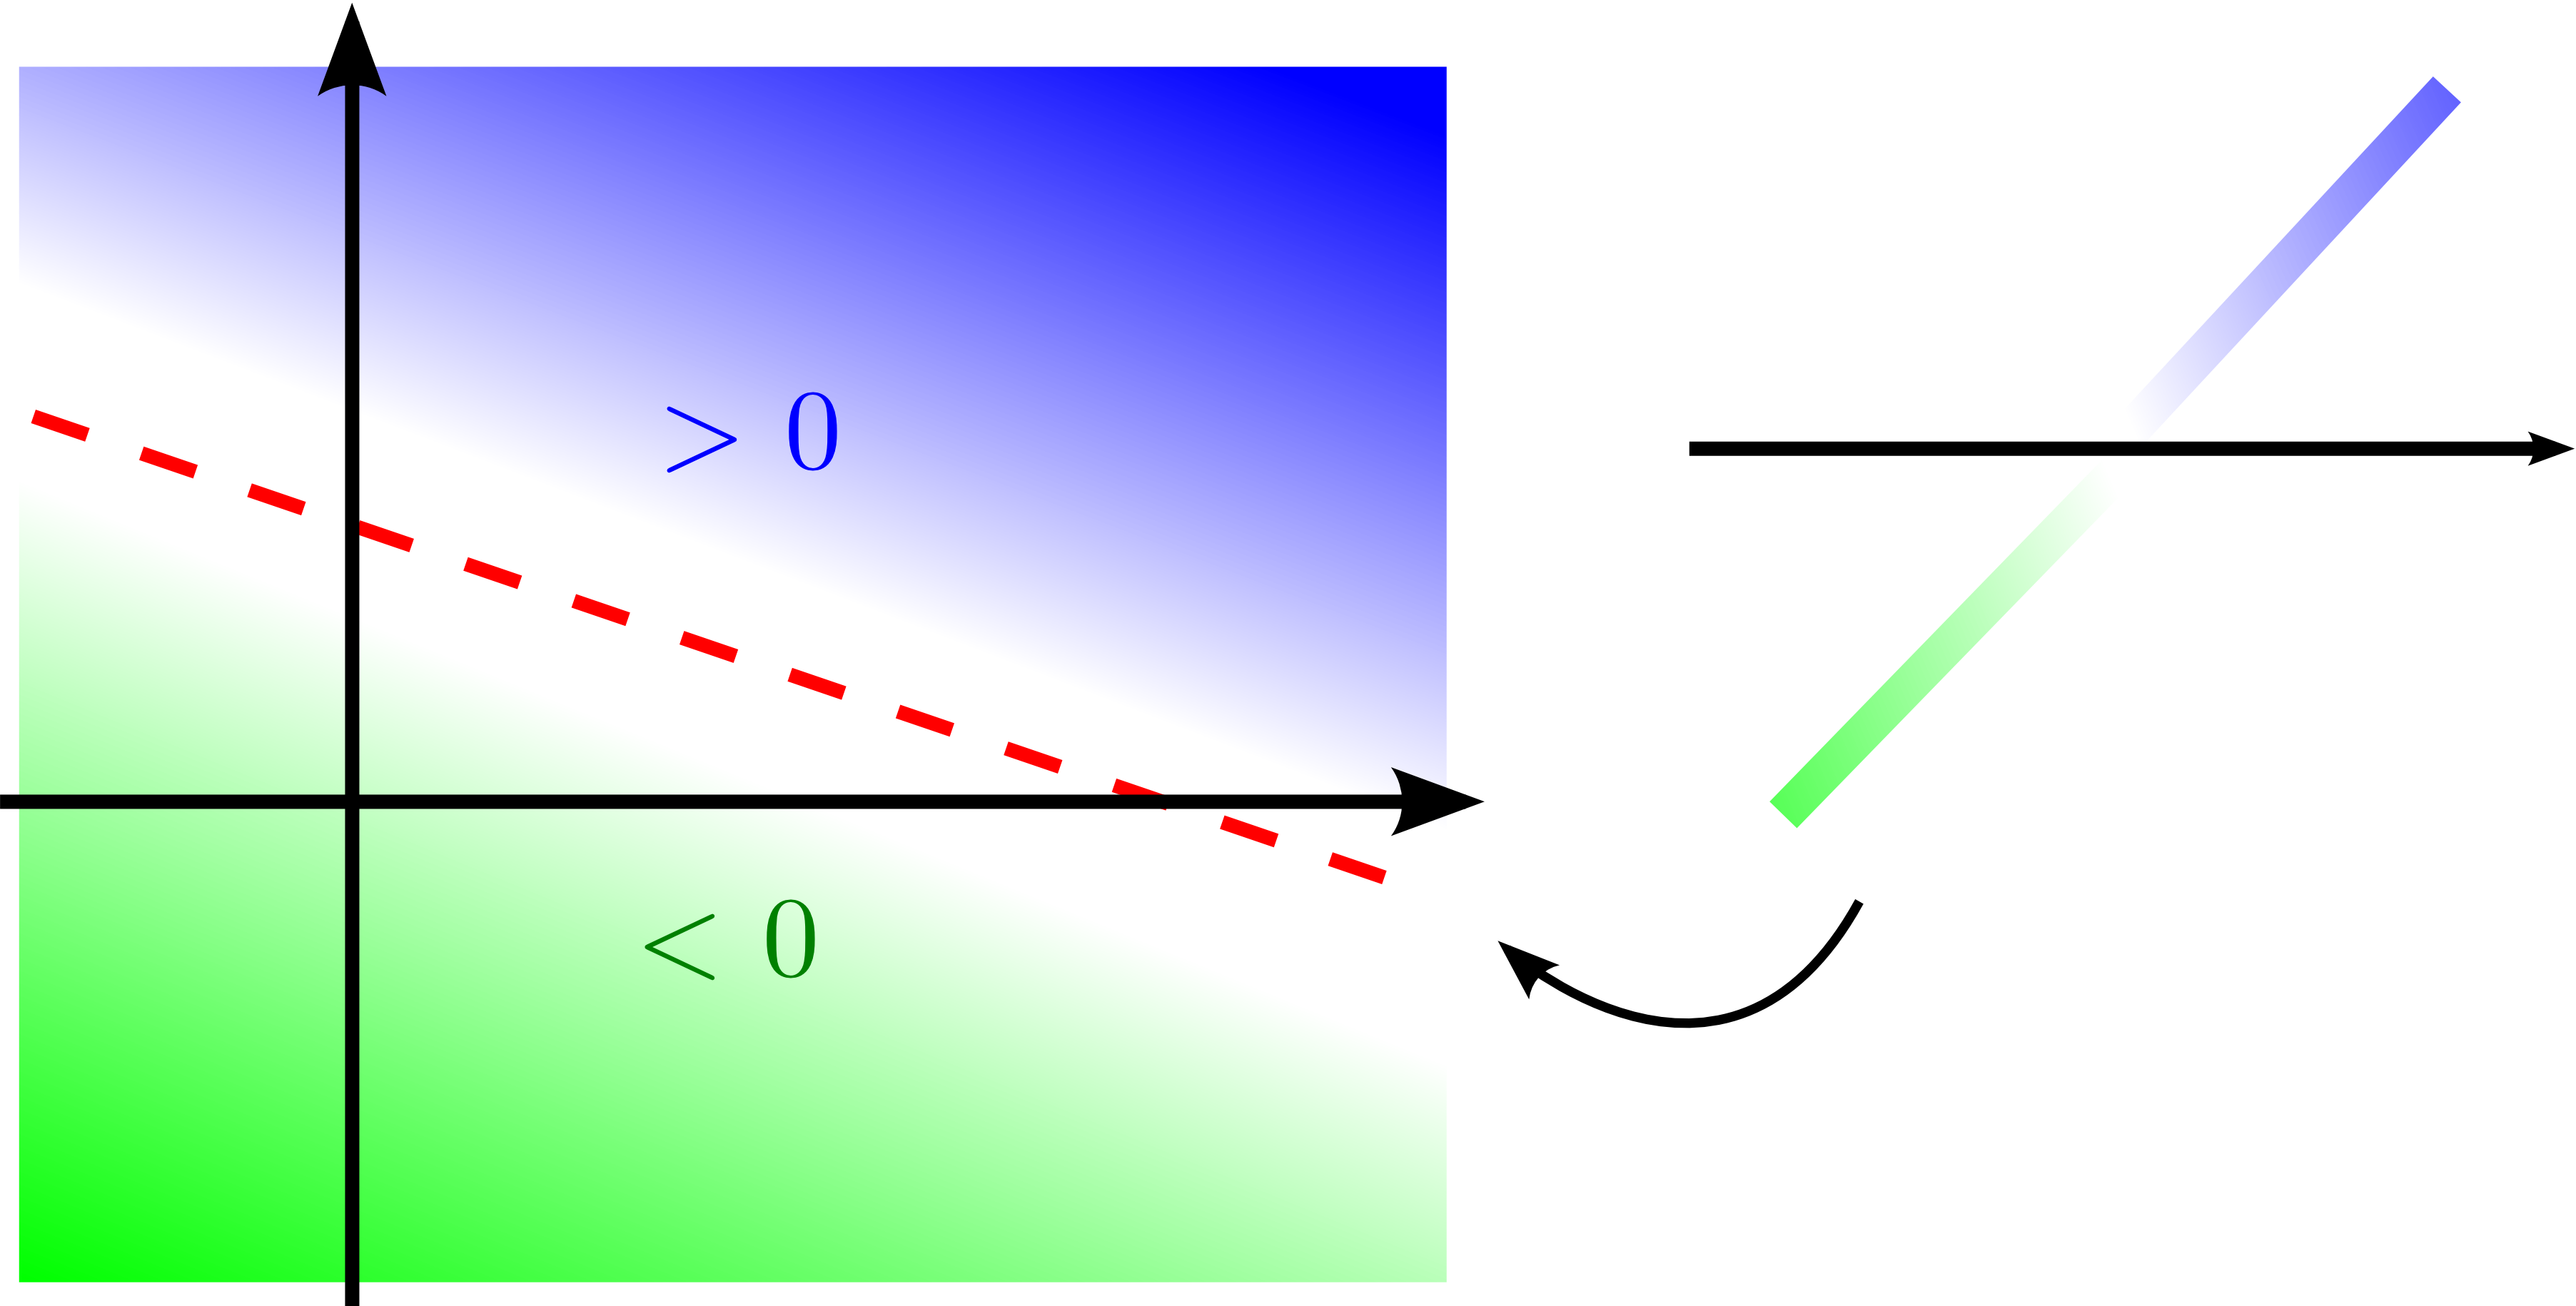
\includegraphics[scale=0.6]{linear-inequality-3.png}}}
\end{equation}
When $\sigmoid$ is applied, 1 represents ``yes'' and 0 represents ``no'', so the contrast between the 2 sides is enhanced, ie, more \textbf{polarized}, or binary:
\begin{equation}
\vcenter{\hbox{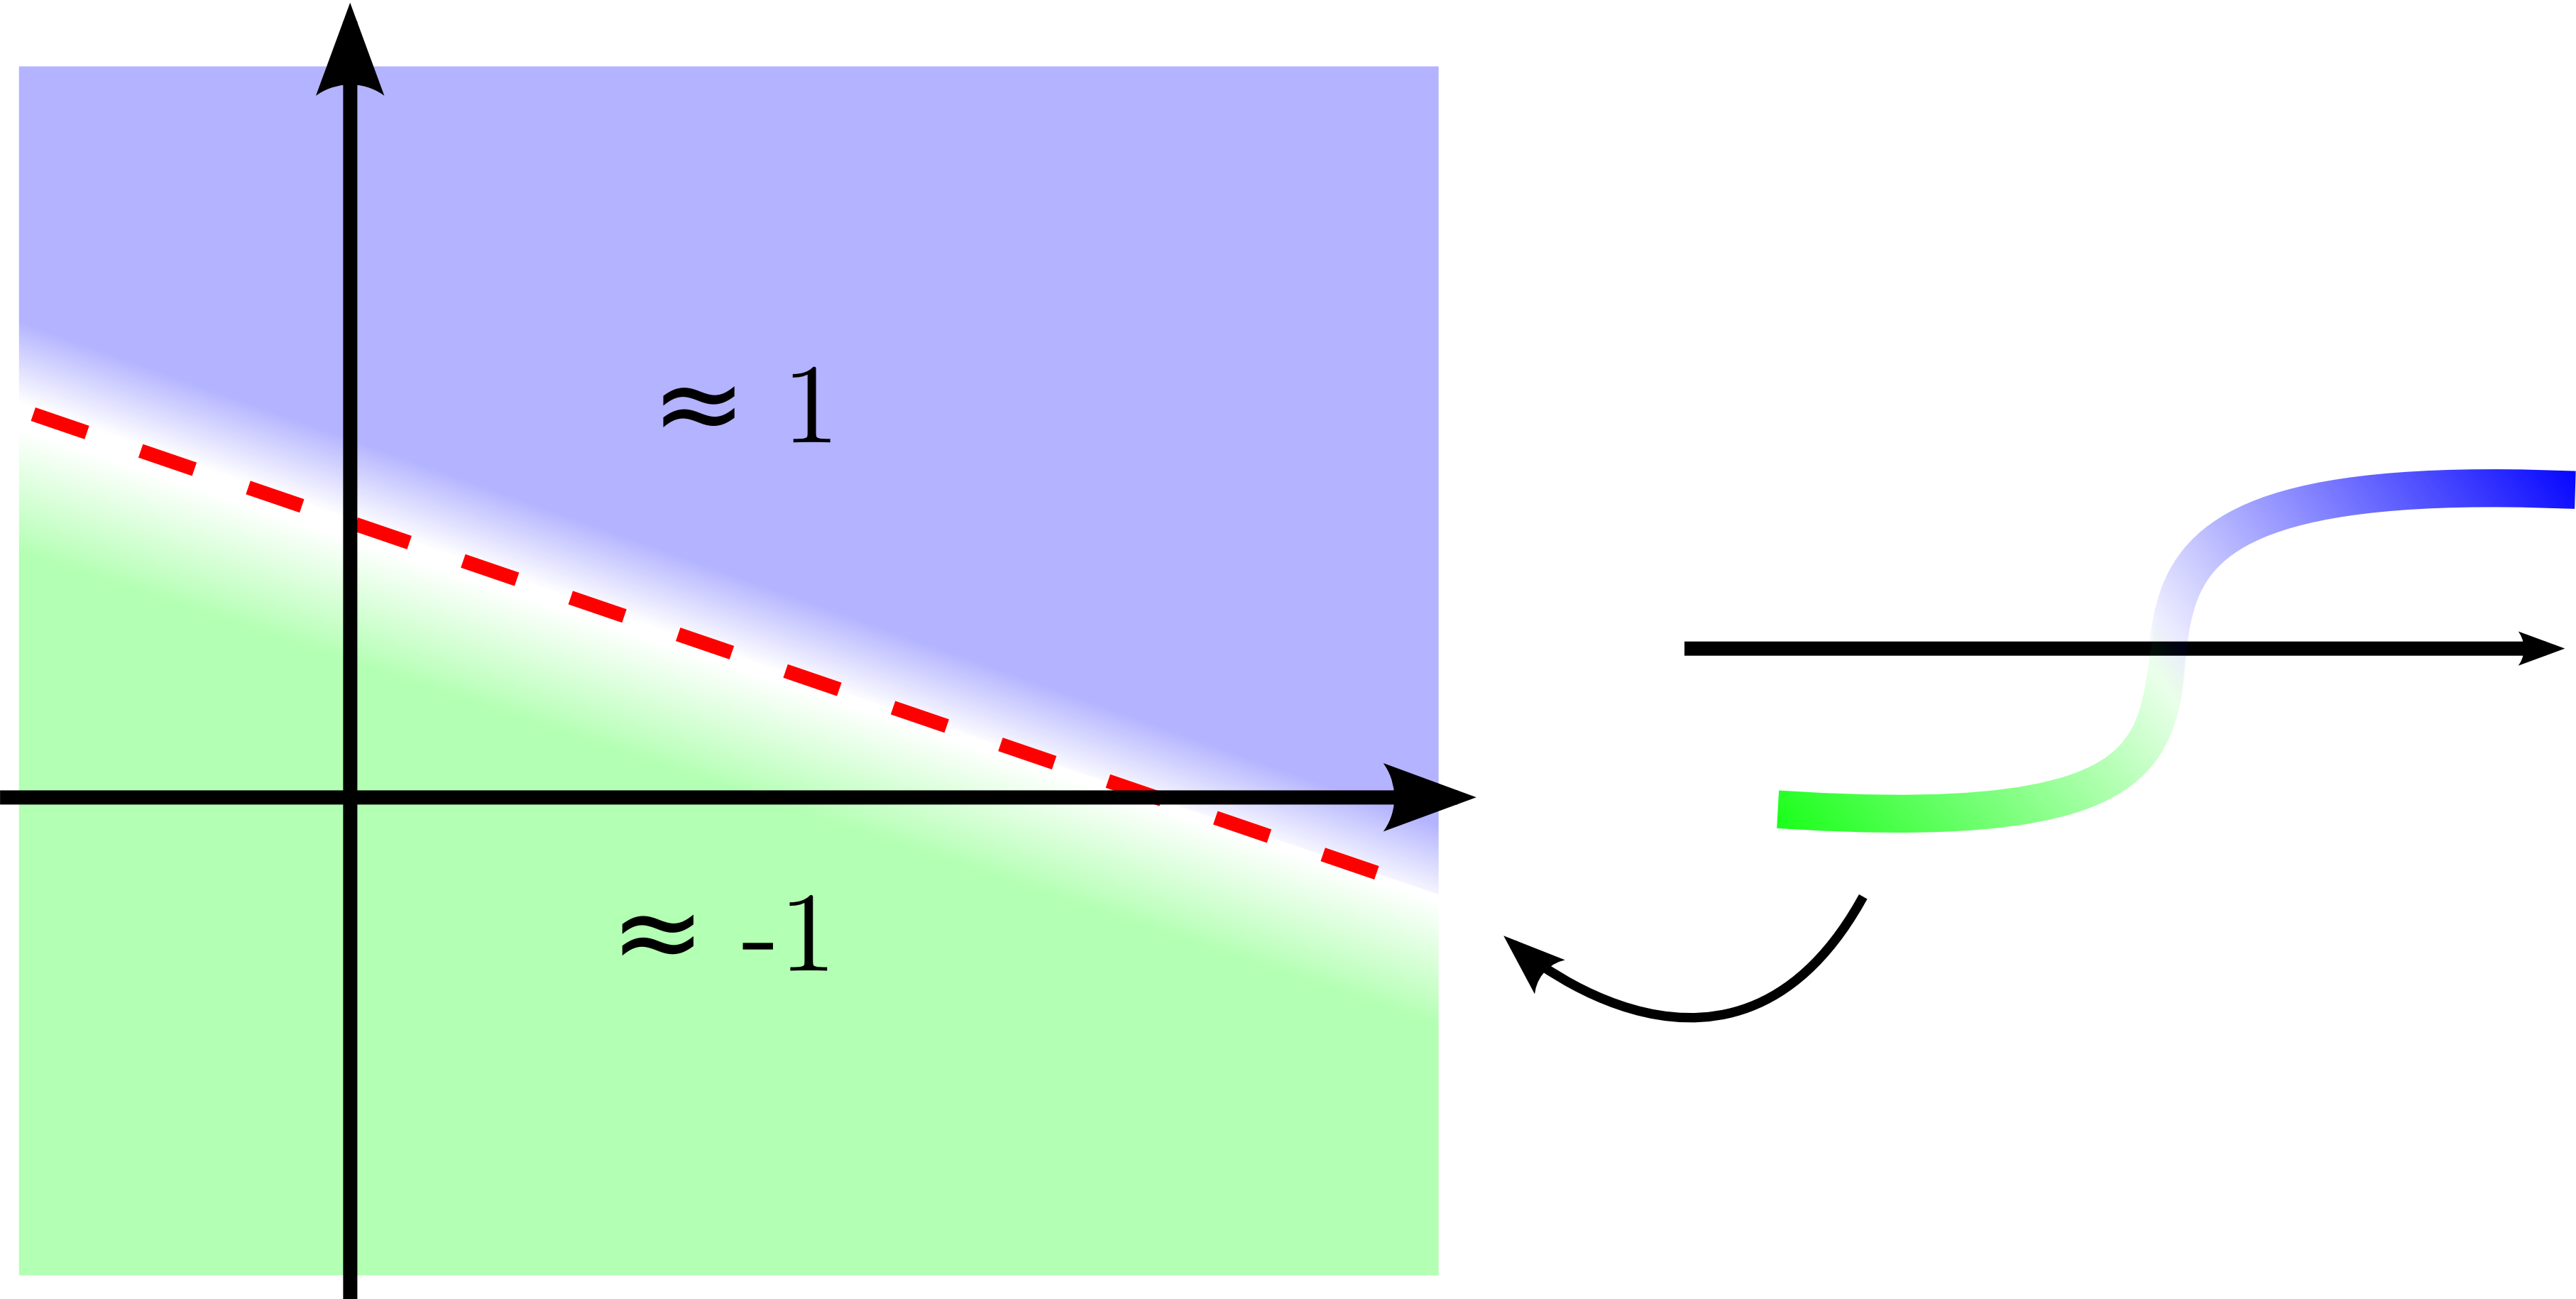
\includegraphics[scale=0.6]{linear-inequality-4.png}}}
\end{equation}

\section*{> 1 neuron}

If there are $> 1$ neurons (on the same layer), eg. 3:
\begin{equation}
\vcenter{\hbox{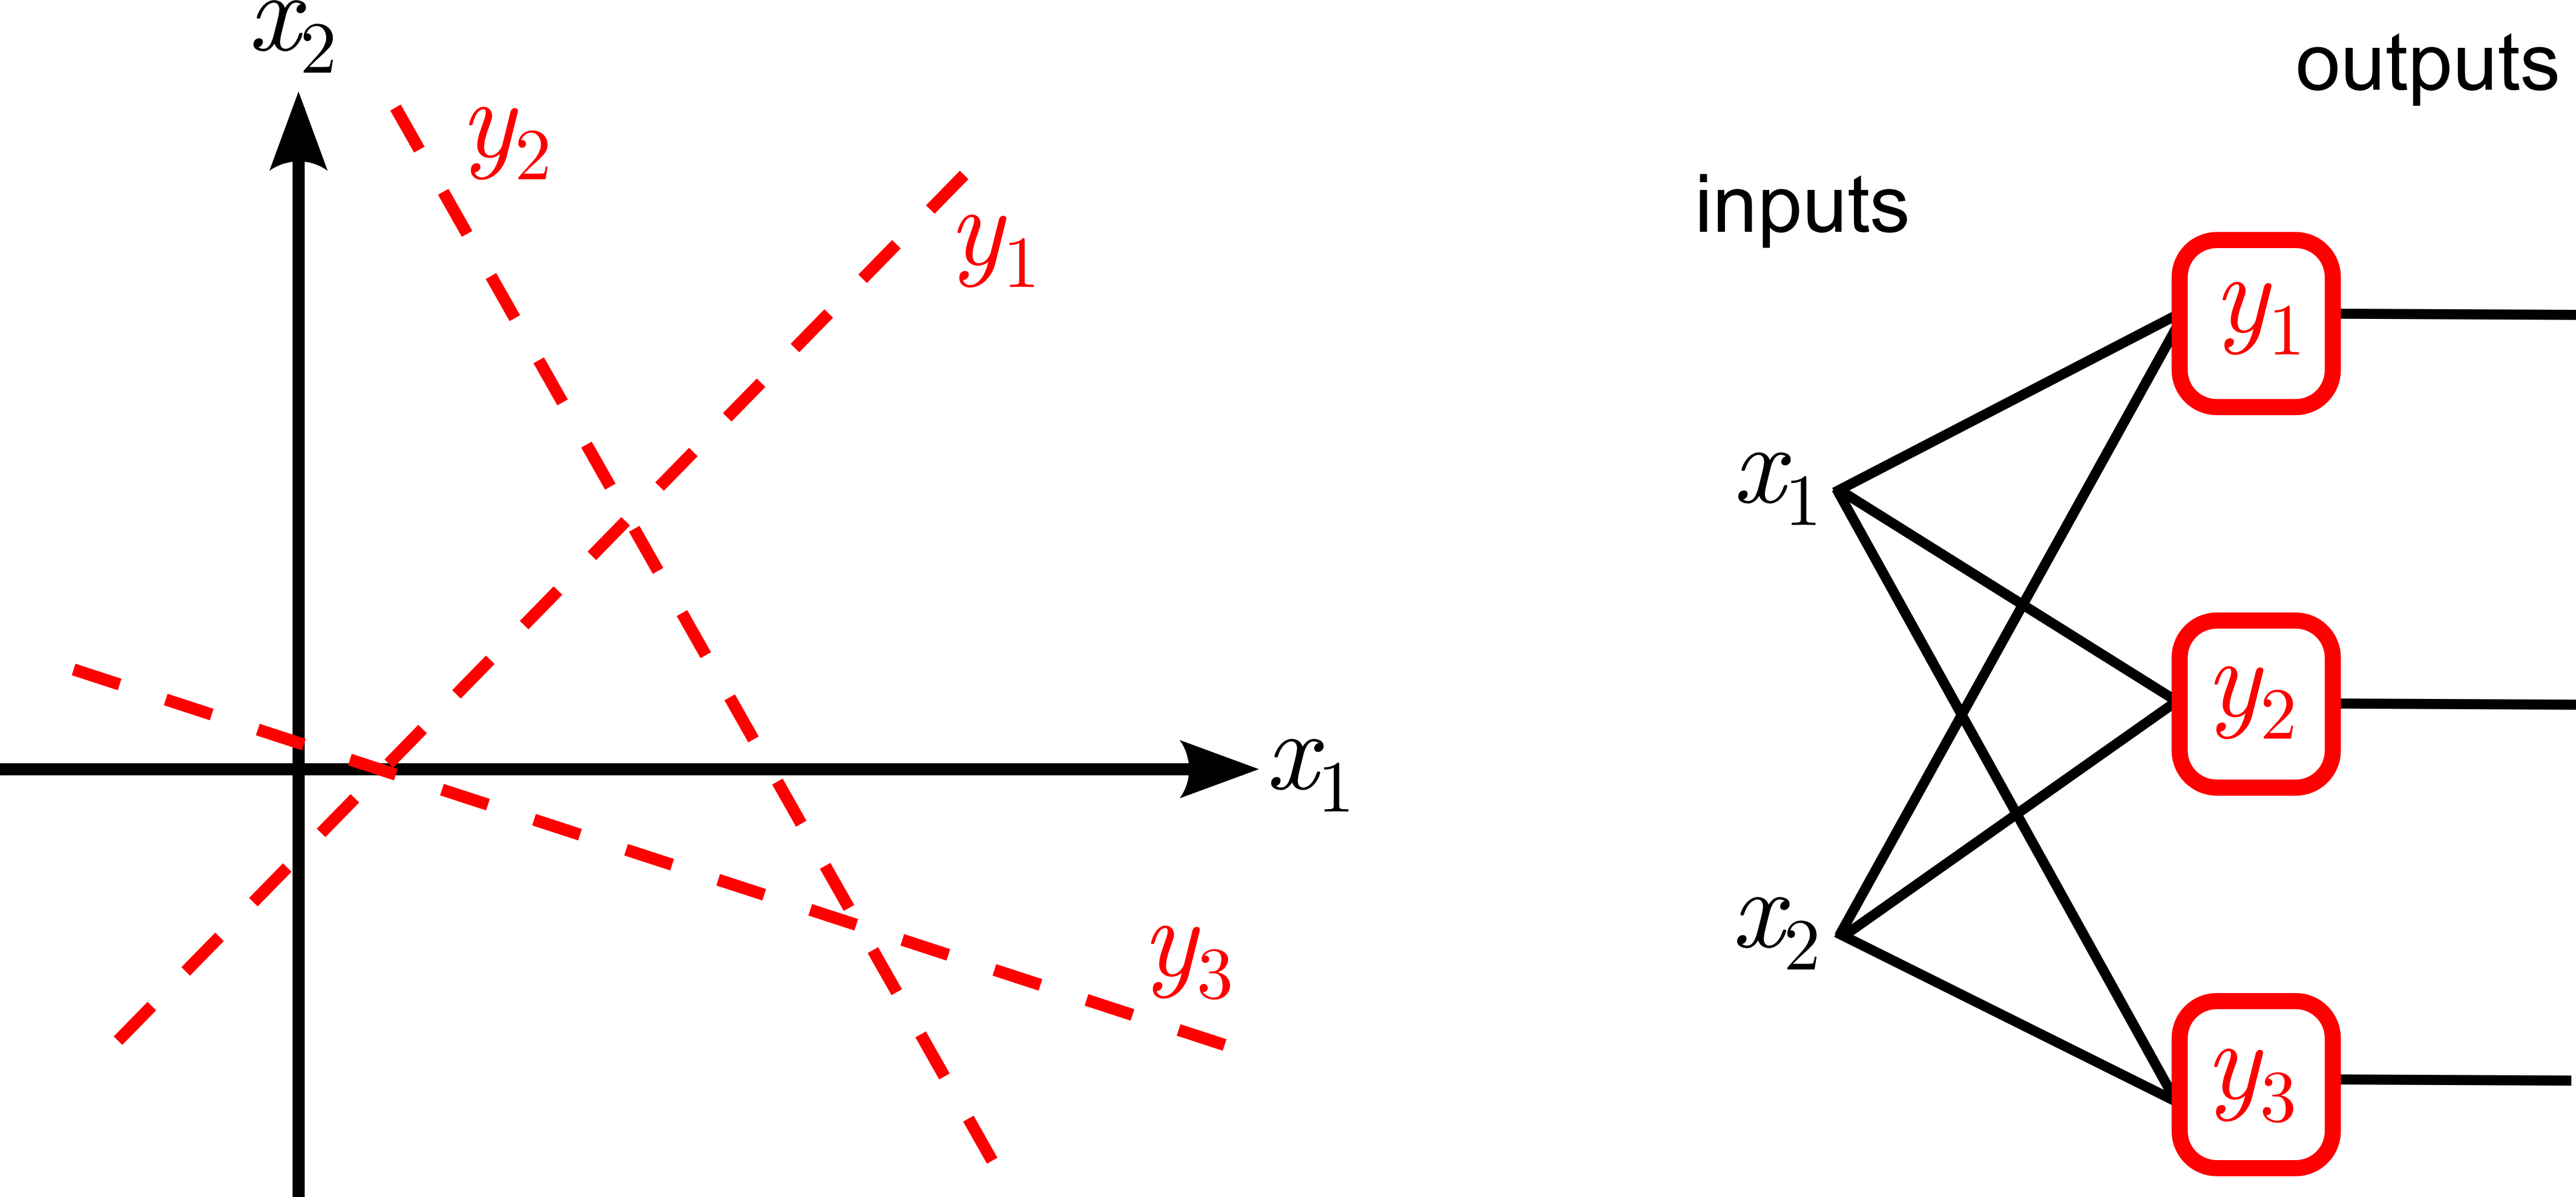
\includegraphics[scale=0.6]{linear-inequalities-1.png}}}
\label{simple-network-layer}
\end{equation}
Note:  The coordinates are $(x_1, x_2) = $ input.  Output is $(y_1, y_2, y_3)$, represented by 3 {\color{red}{dotted}} lines.  The \textbf{network topology} of this \textbf{1 layer} of neural network is as shown on the right (The $\sum$ and $\sigmoid$ for each neuron are not shown).

Each neuron may choose one side to be ``yes''.  The \textbf{conjunctions} of these choices may form various shapes, eg:
\begin{equation}
\vcenter{\hbox{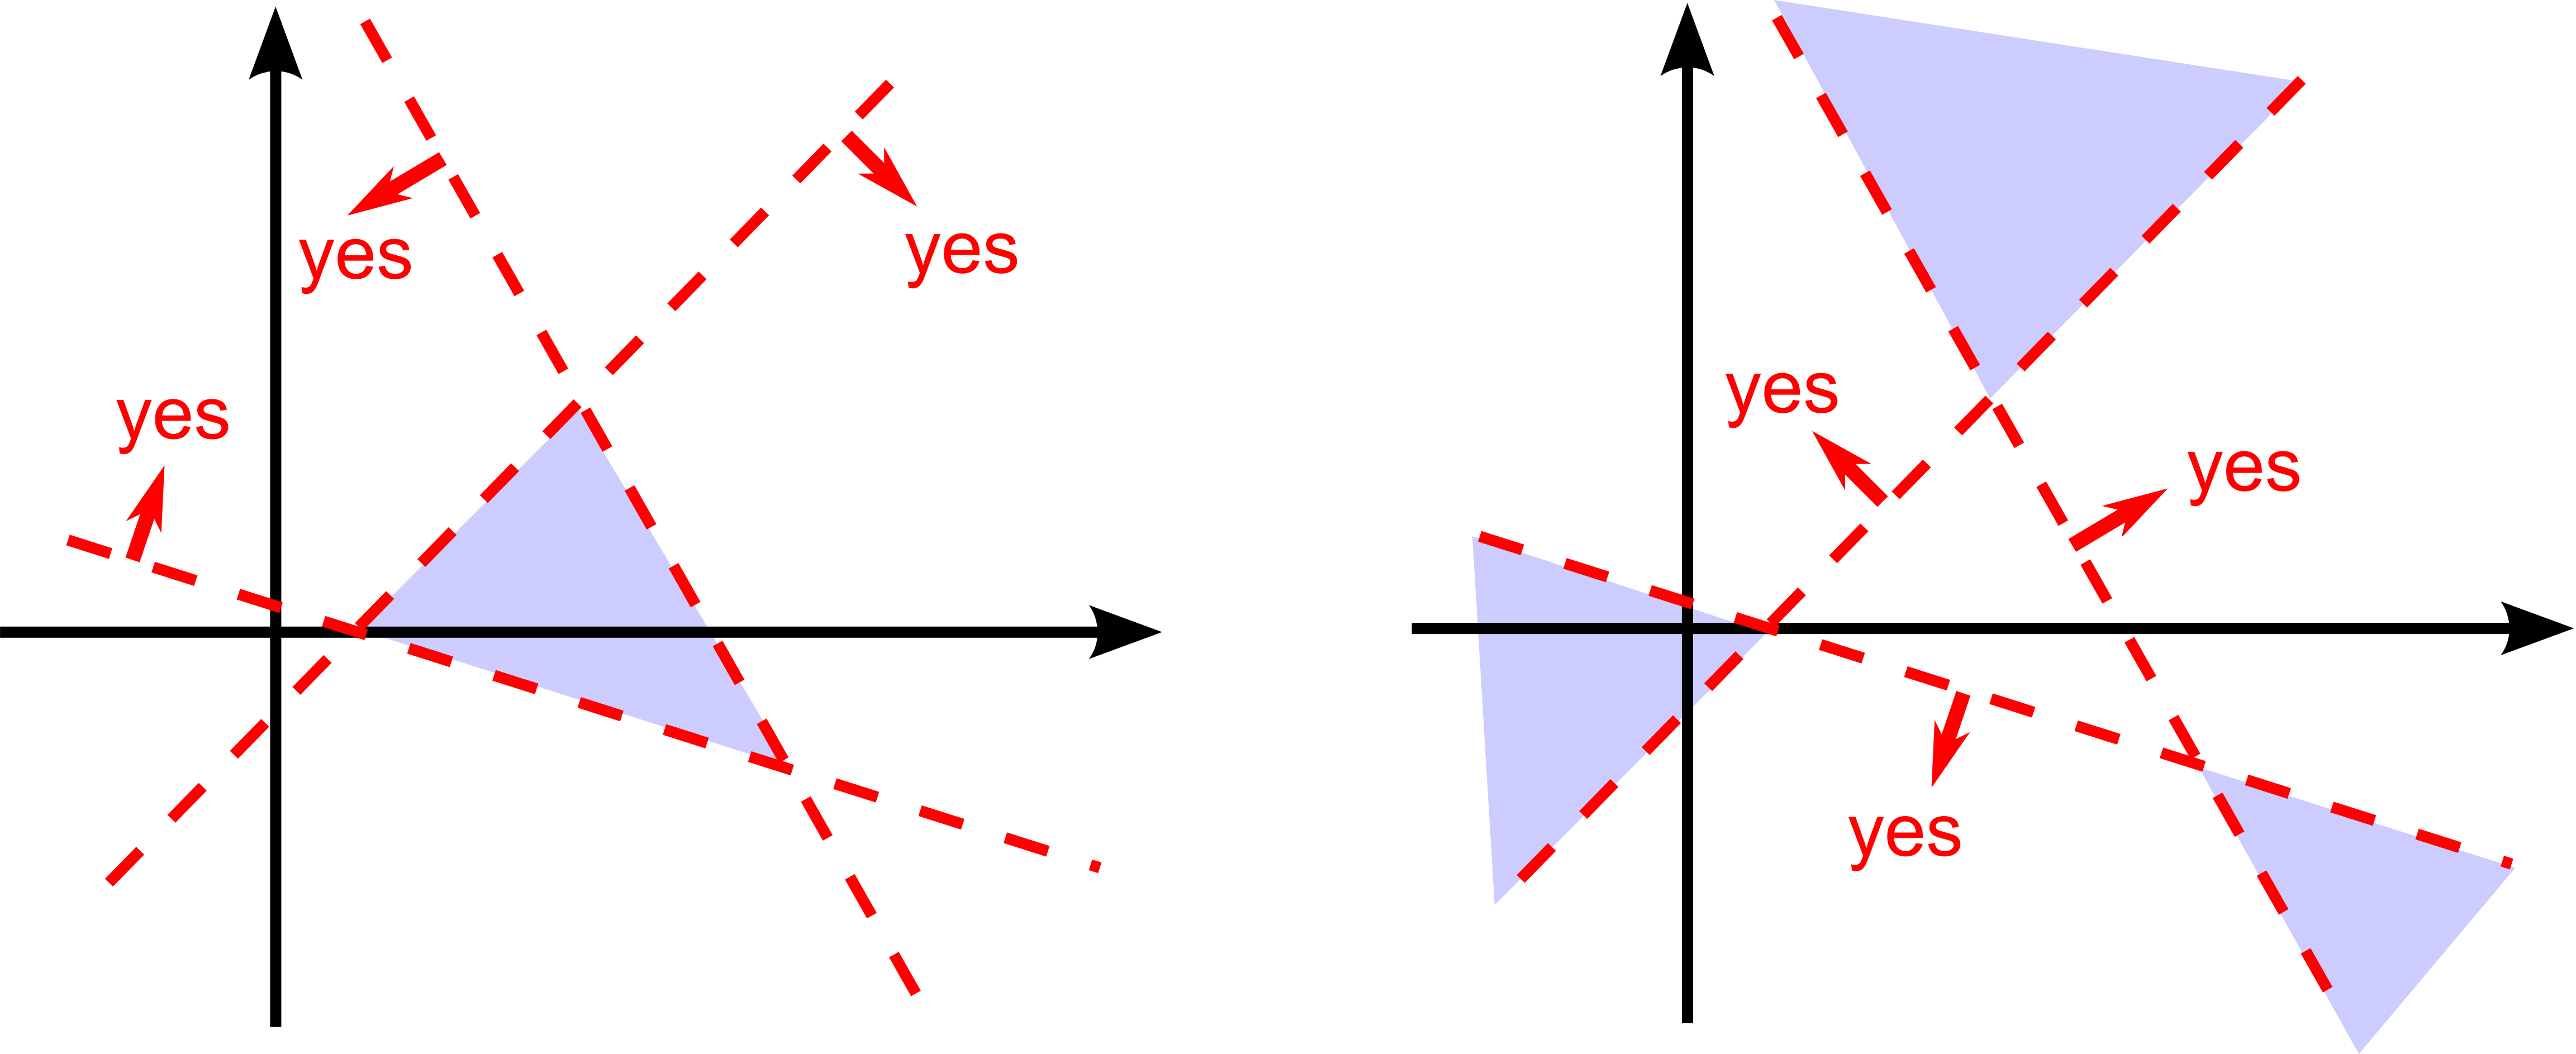
\includegraphics[scale=0.6]{linear-inequalities-2.png}}}
\end{equation}
Also notice that in the right figure, a number of disjoint regions (separated in space) are possible.

Obviously, we could use neurons to separate and classify points in space, thus achieving the goal of \textbf{machine learning}.

\section*{1 layer of neurons}

%简单来说,当神经网络的\textbf{层数}增加,在输入空间的切割形状会变得更为\textbf{复杂},所以多层的神经网络有能力学习出非常复杂的 patterns,这就是\textbf{深度学习}的优势。

In this part we need more \textbf{linear algebra}, which I will explain in another tutorial.

The mathematical form of 1 layer of neural network is:
\begin{equation}
\boxed{output} \; \vect{y} = \sigmoid [ W \vect{x} ] 
\end{equation}
where $W$ is a matrix, ie. a \textbf{linear transformation}; $\sigmoid$ is a \textbf{non-linear transformation}.

Matrices are a compact way of writing \textbf{systems of linear equations}.  1 neuron = $\sigmoid \circ \boxed{linear combination}$, each linear combination is a \textbf{row} in a matrix.

Every matrix is a representation for a \textbf{linear transformation}:
\begin{equation}
\vcenter{\hbox{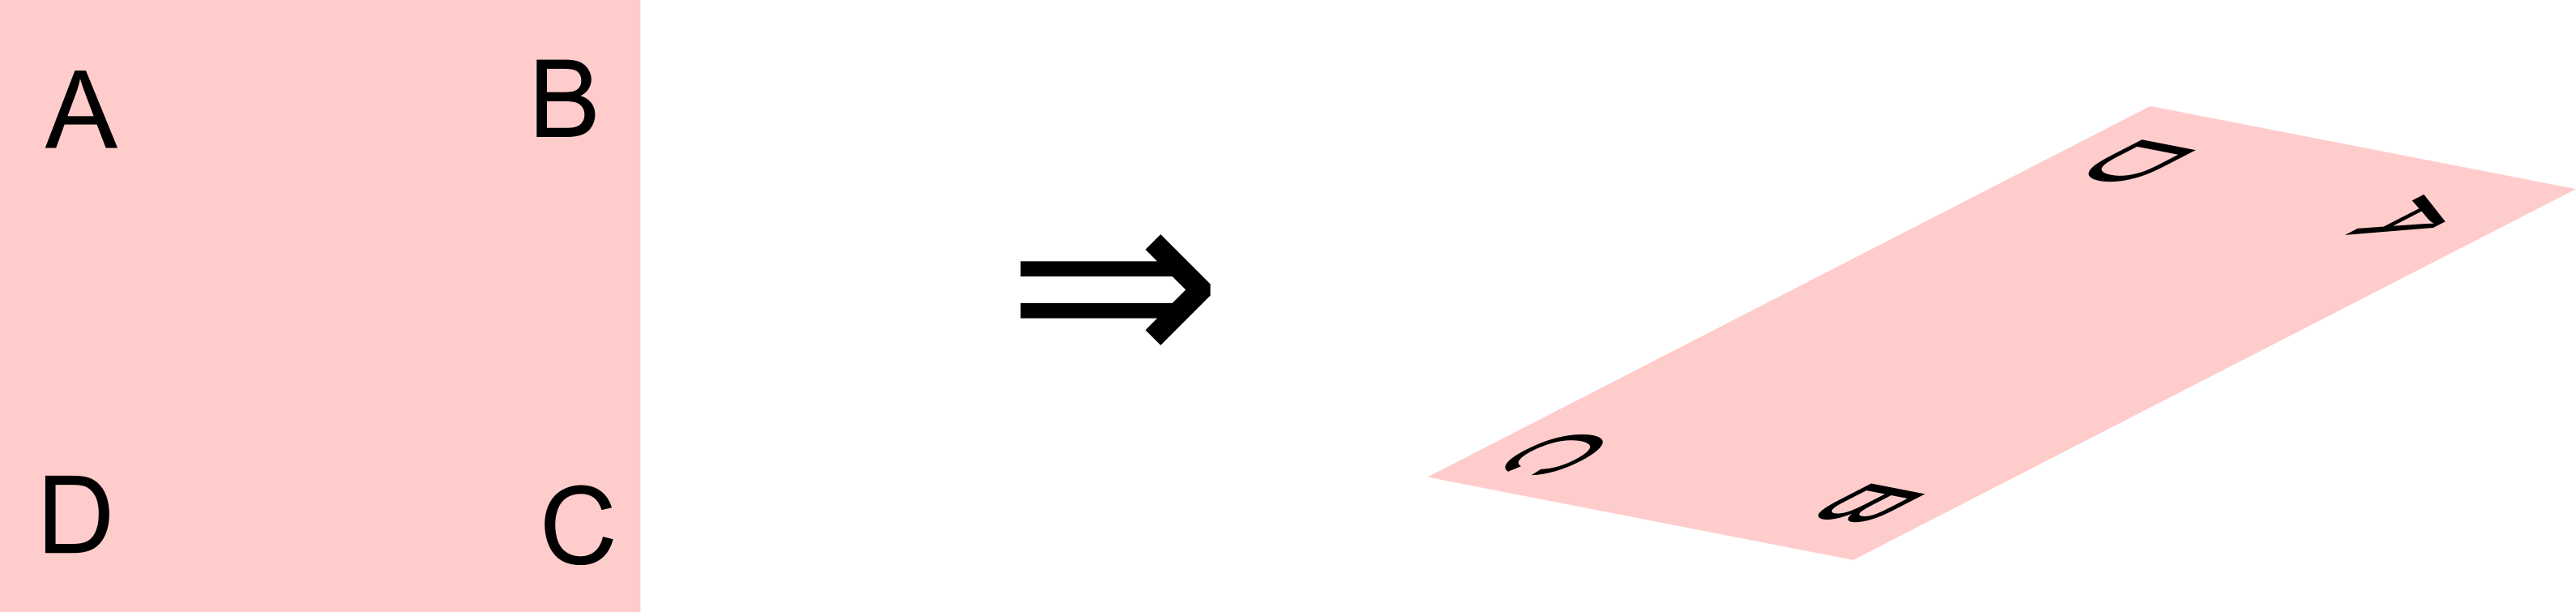
\includegraphics[scale=0.6]{linear-transformation.png}}}
\end{equation}
Linear transformations can ``skew'' a square into a parallelogram, and also include \textbf{rotations} and \textbf{translations}.  Straight lines are preserved as straight lines, hence its name.

Next we need to know what $\sigmoid$ does:  (below is the sigmoid transform of both $x$ and $y$ coordinates)
\begin{equation}
\vcenter{\hbox{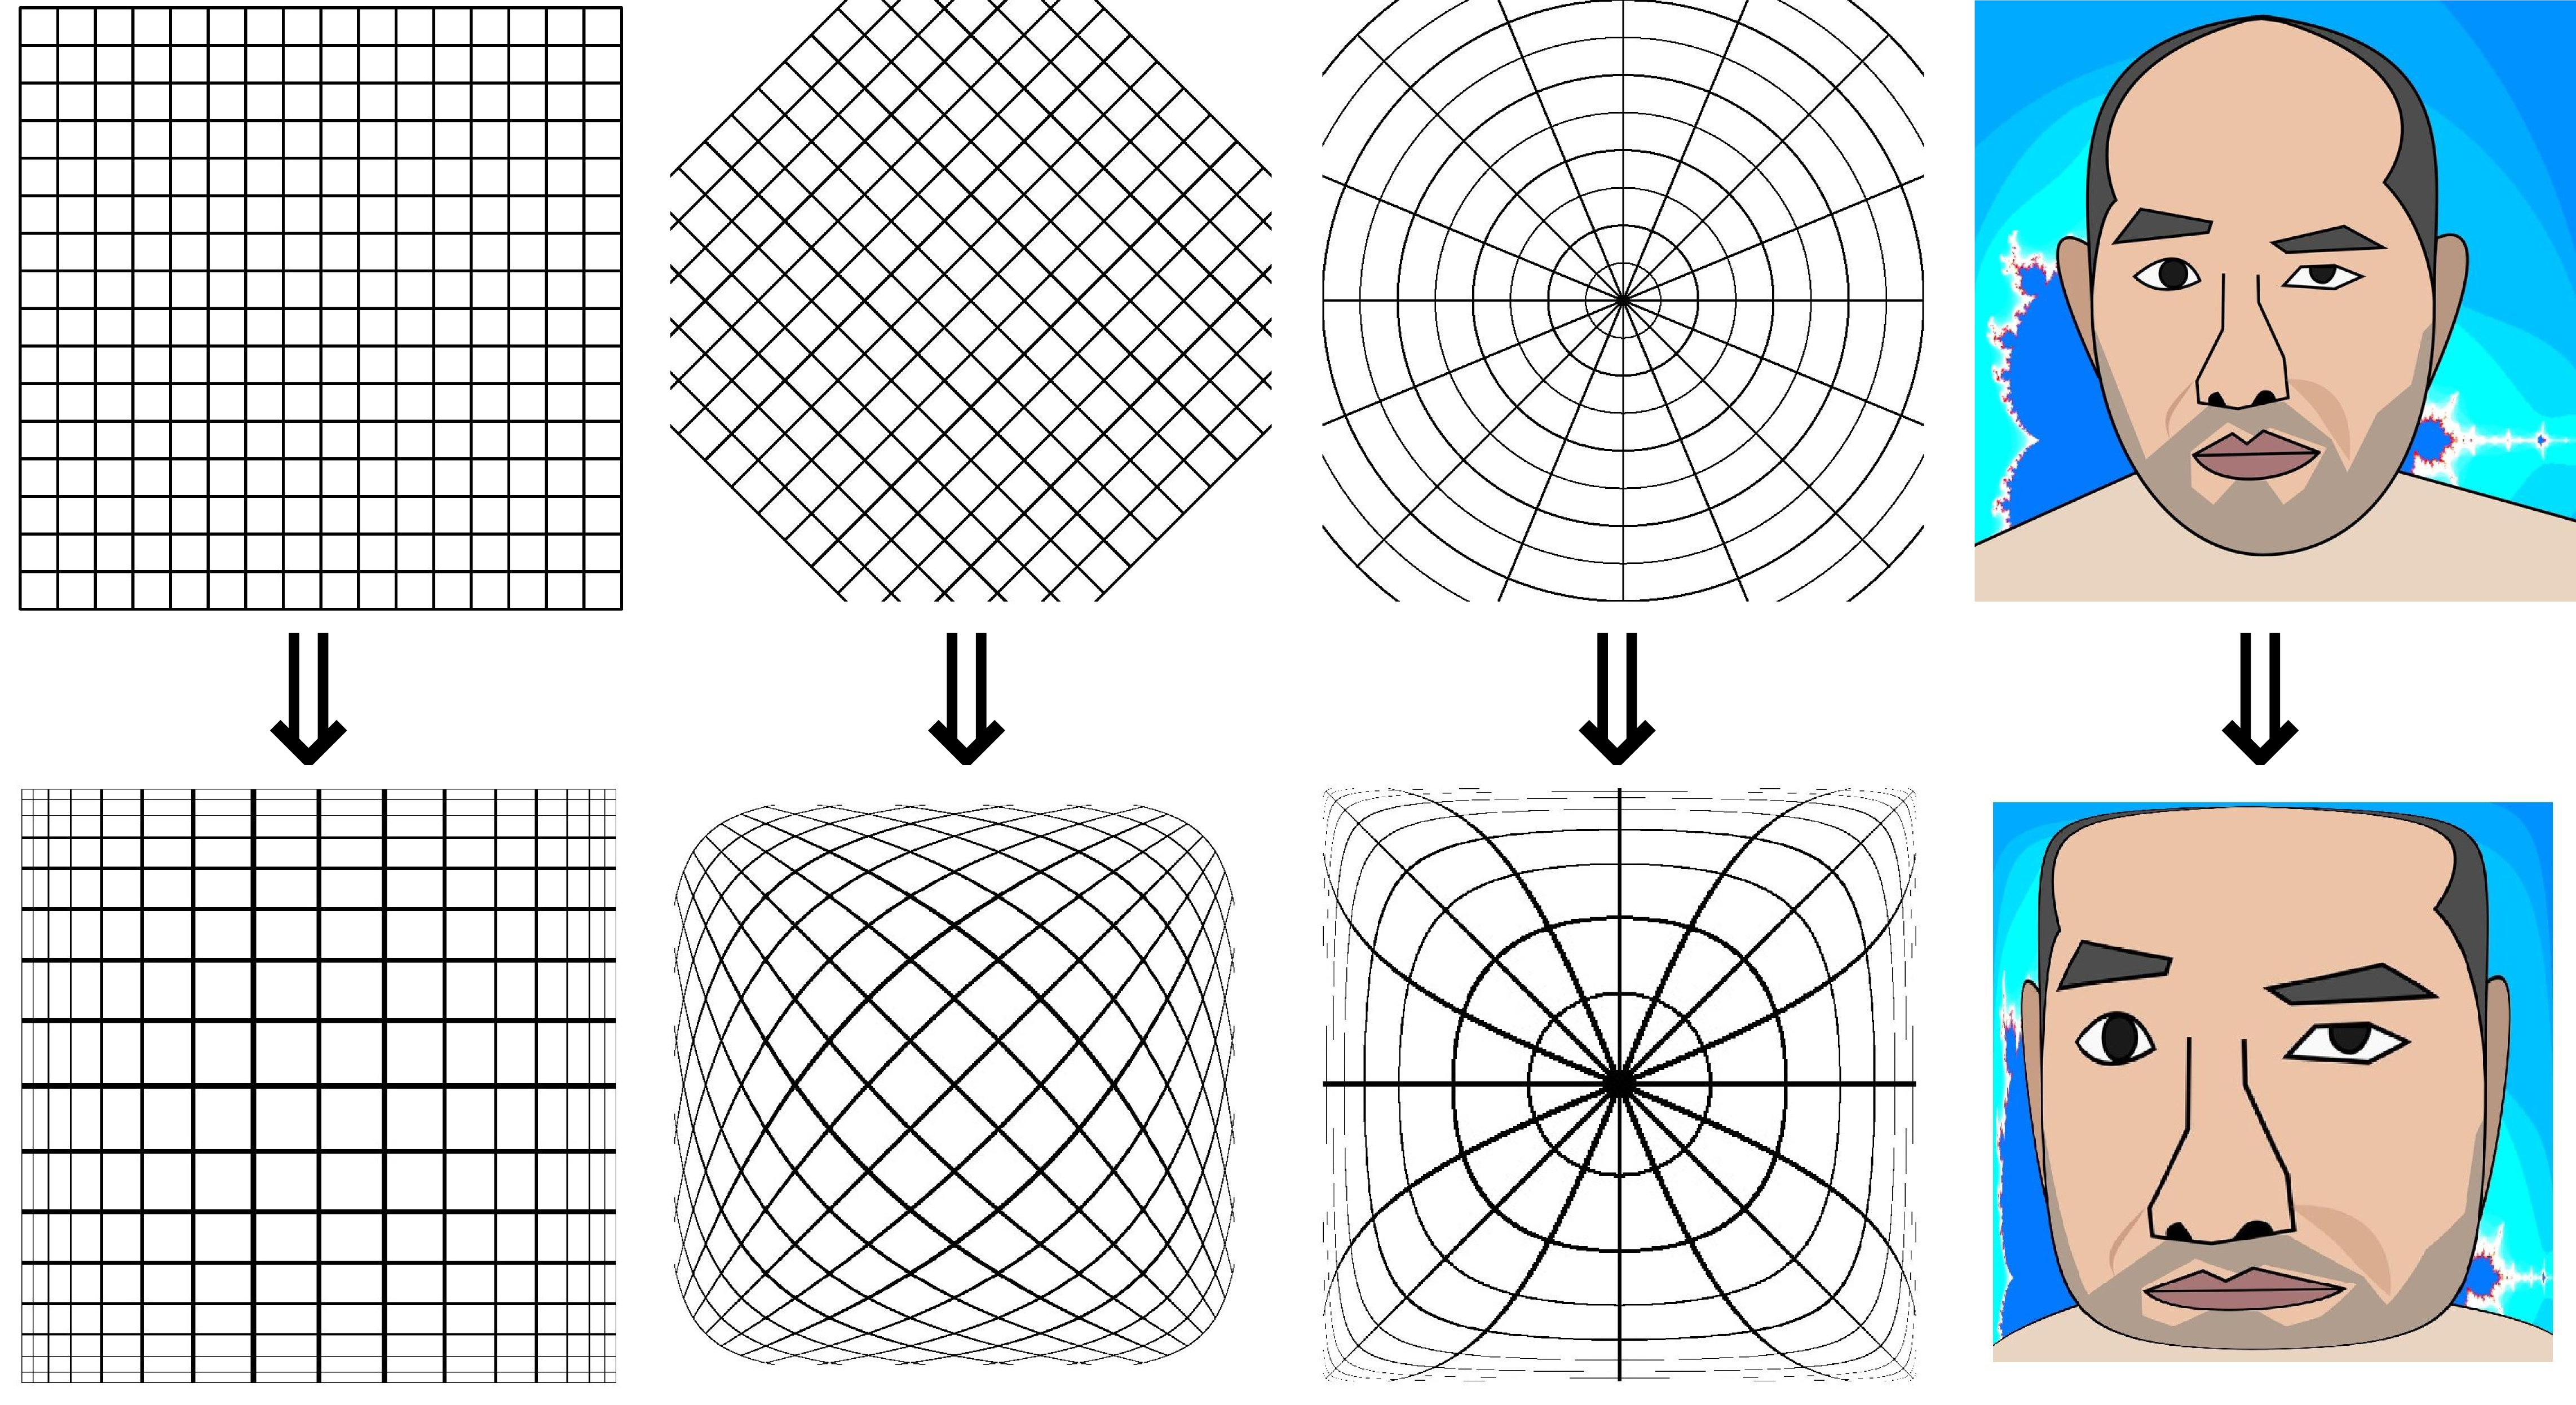
\includegraphics[scale=0.75]{sigmoid-transforms.png}}}
\end{equation}
$\sigmoid$ can be seen as ``stretching'' the square to its 4 corners, so I take on the ``square-faced'' look.

We say that these vertices are \textbf{attractors}:
\begin{equation}
\vcenter{\hbox{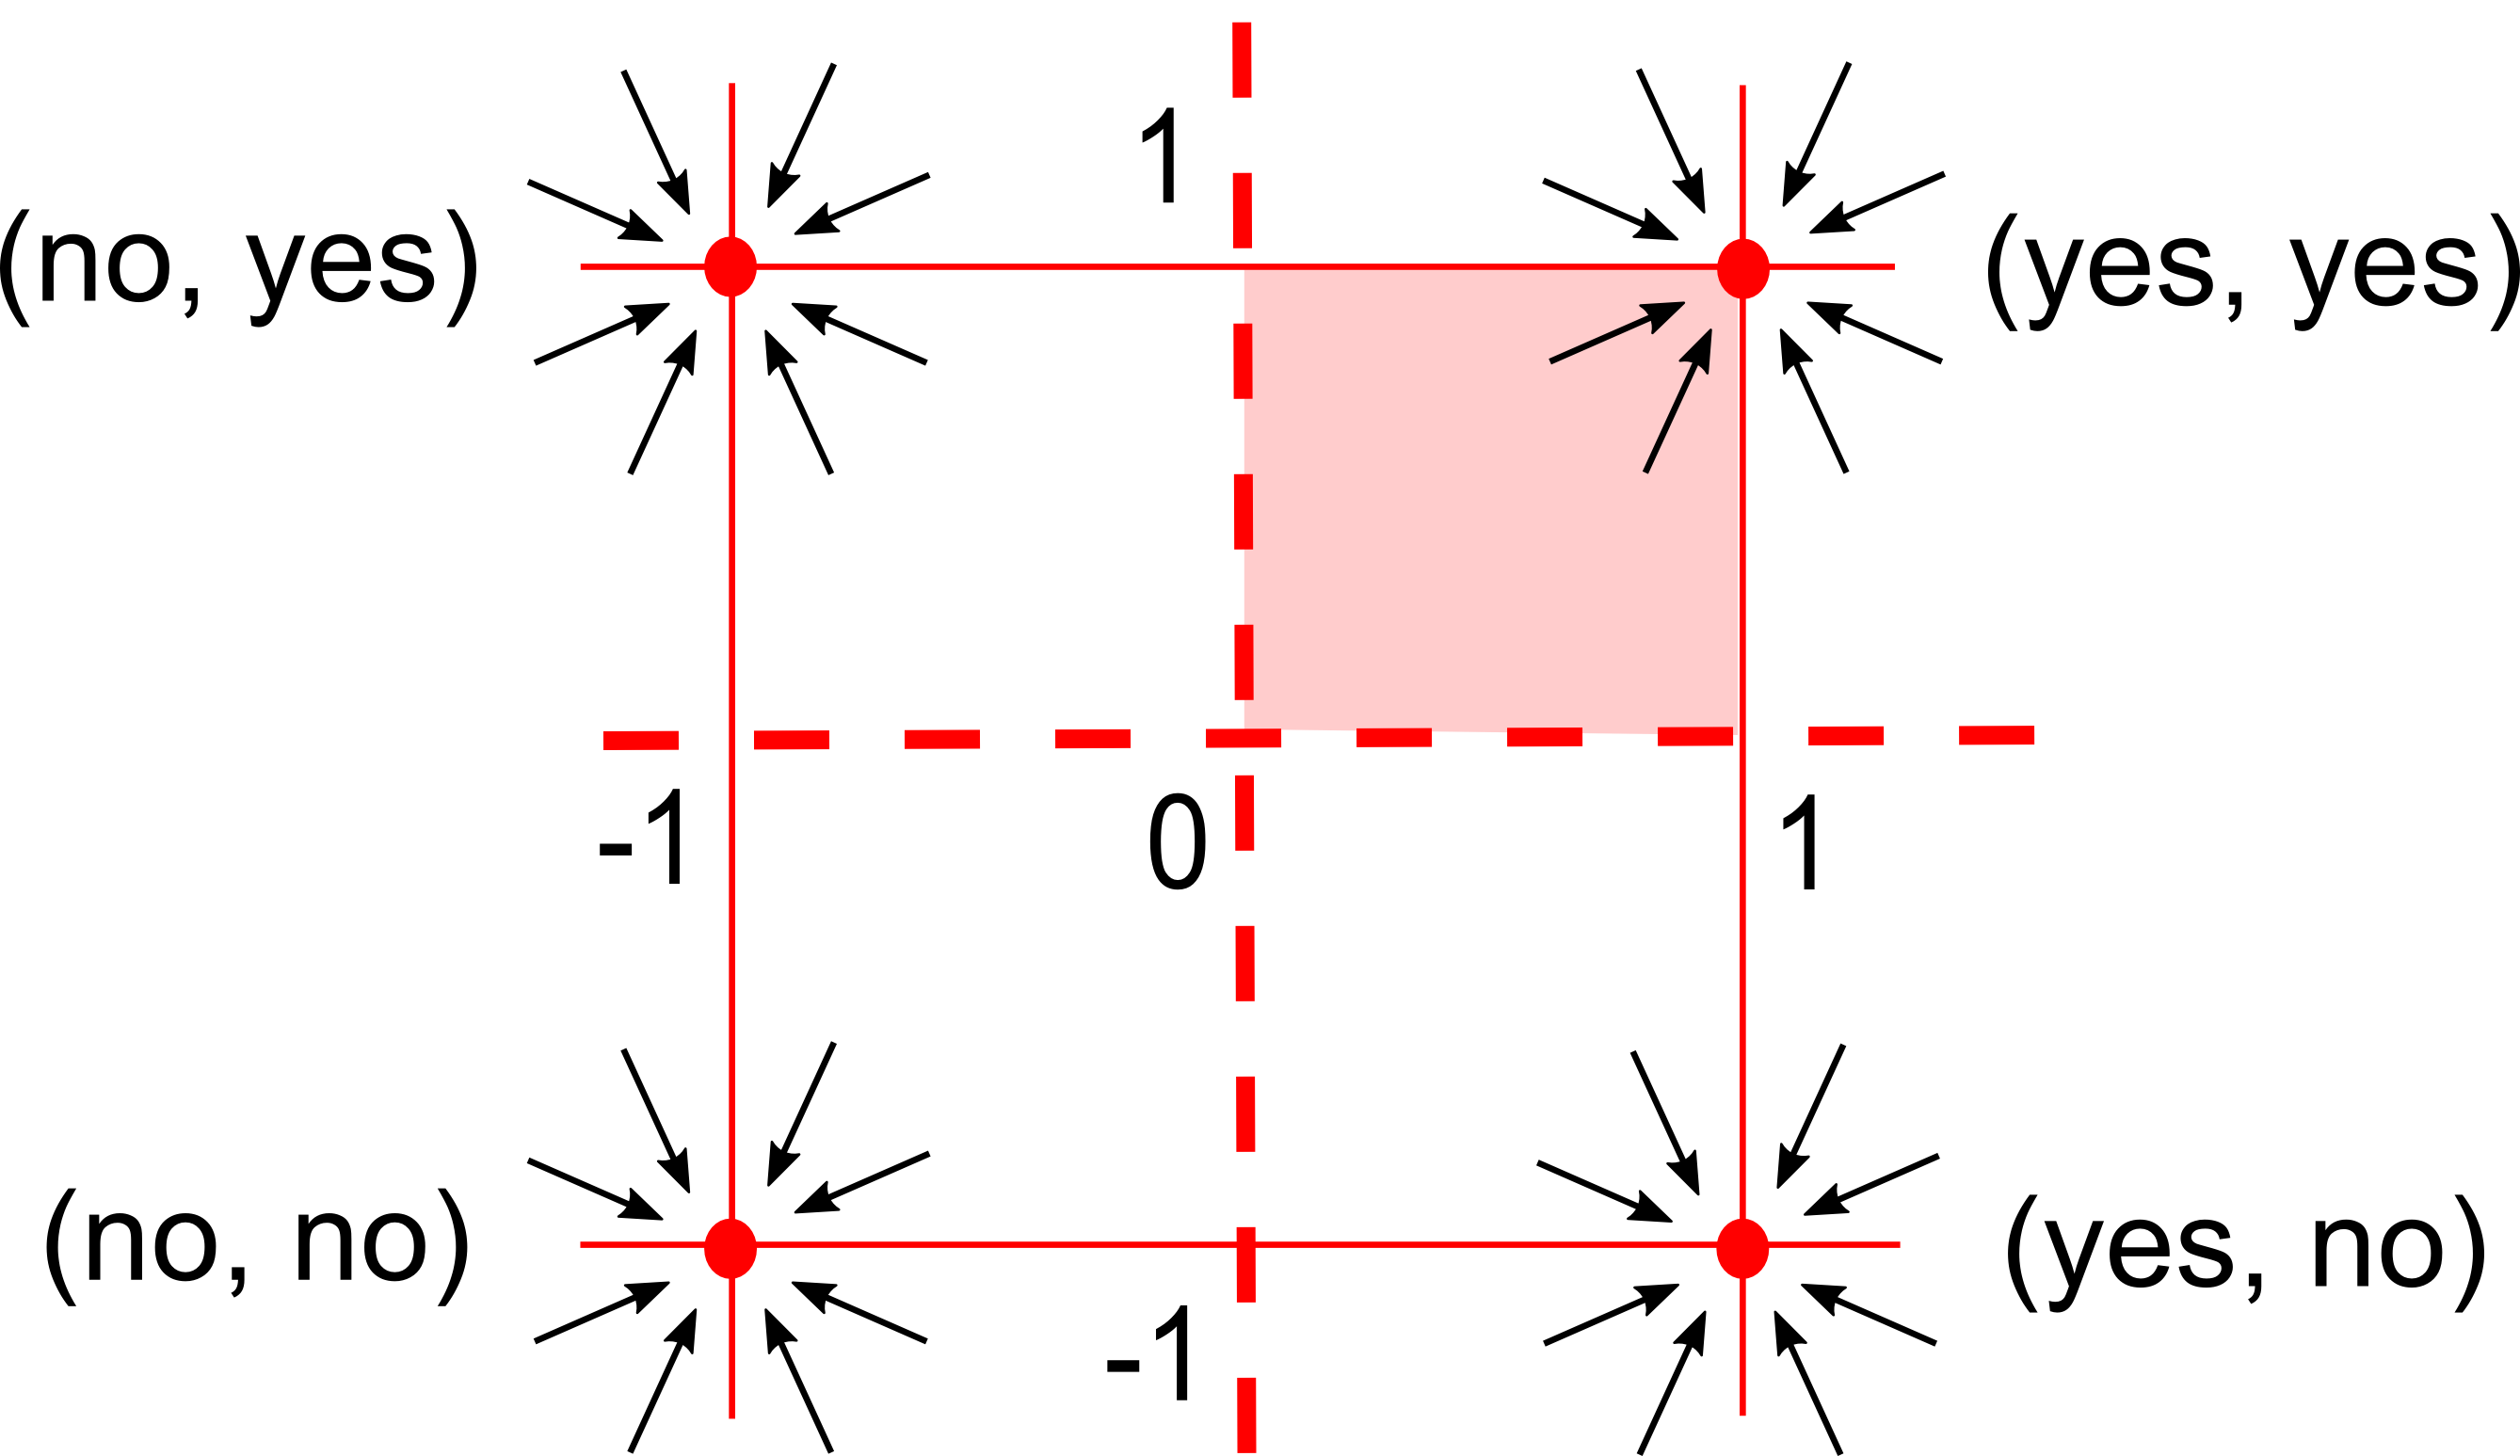
\includegraphics[scale=0.75]{attractors.png}}}
\end{equation}

Note:  During the $\sigmoid$ transform, the image is compressed from the \textbf{infinite} unbounded space to the $[-1,+1]^2$ square:
\begin{equation}
\vcenter{\hbox{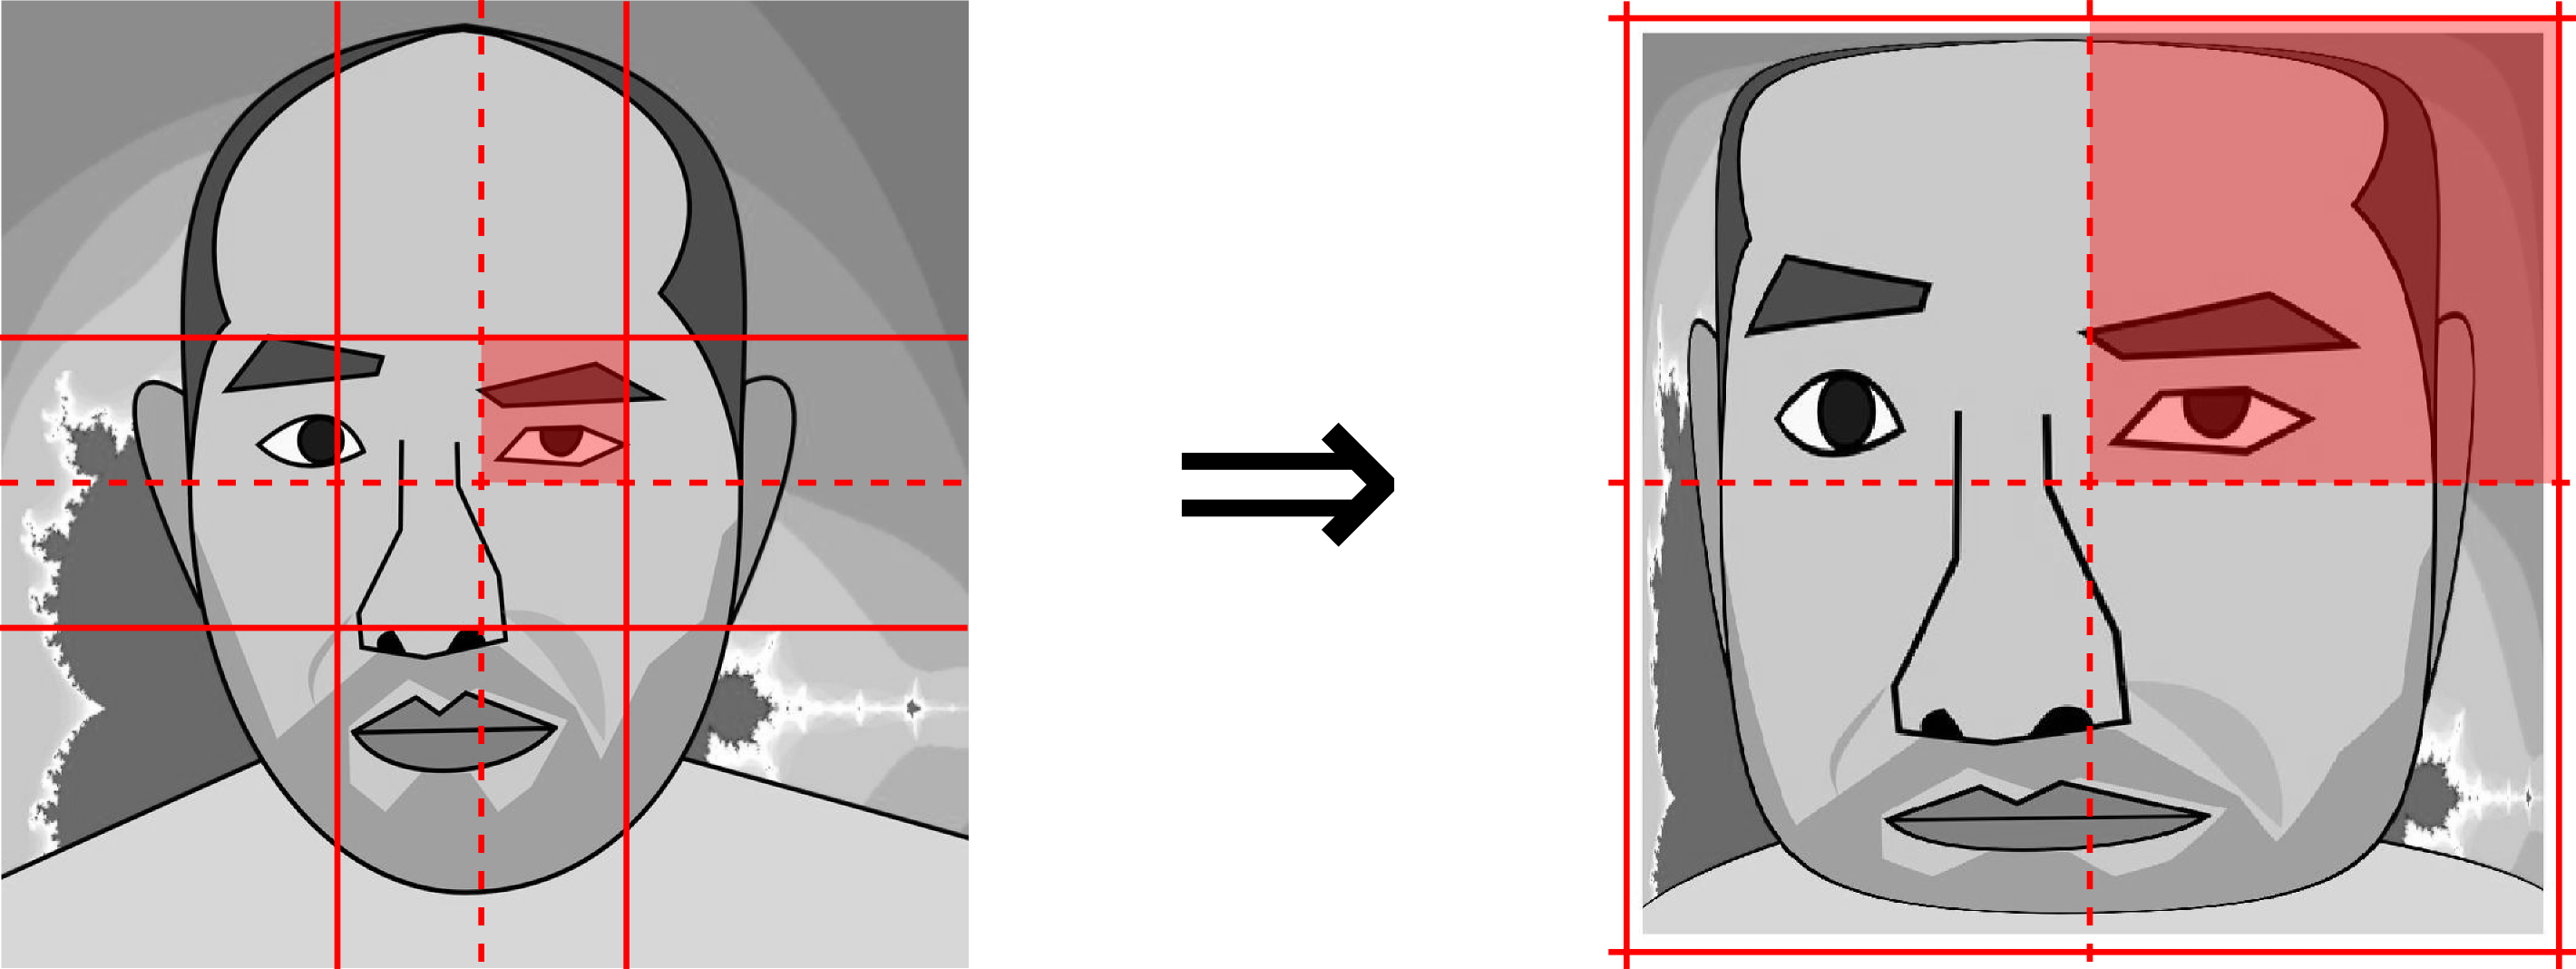
\includegraphics[scale=0.6]{sigmoid-transform-1.png}}}
\end{equation}

Here is the transformation performed by \textbf{1 layer} of neural network, decomposed into the $W$ and $\sigmoid$ parts:
\begin{equation}
\vcenter{\hbox{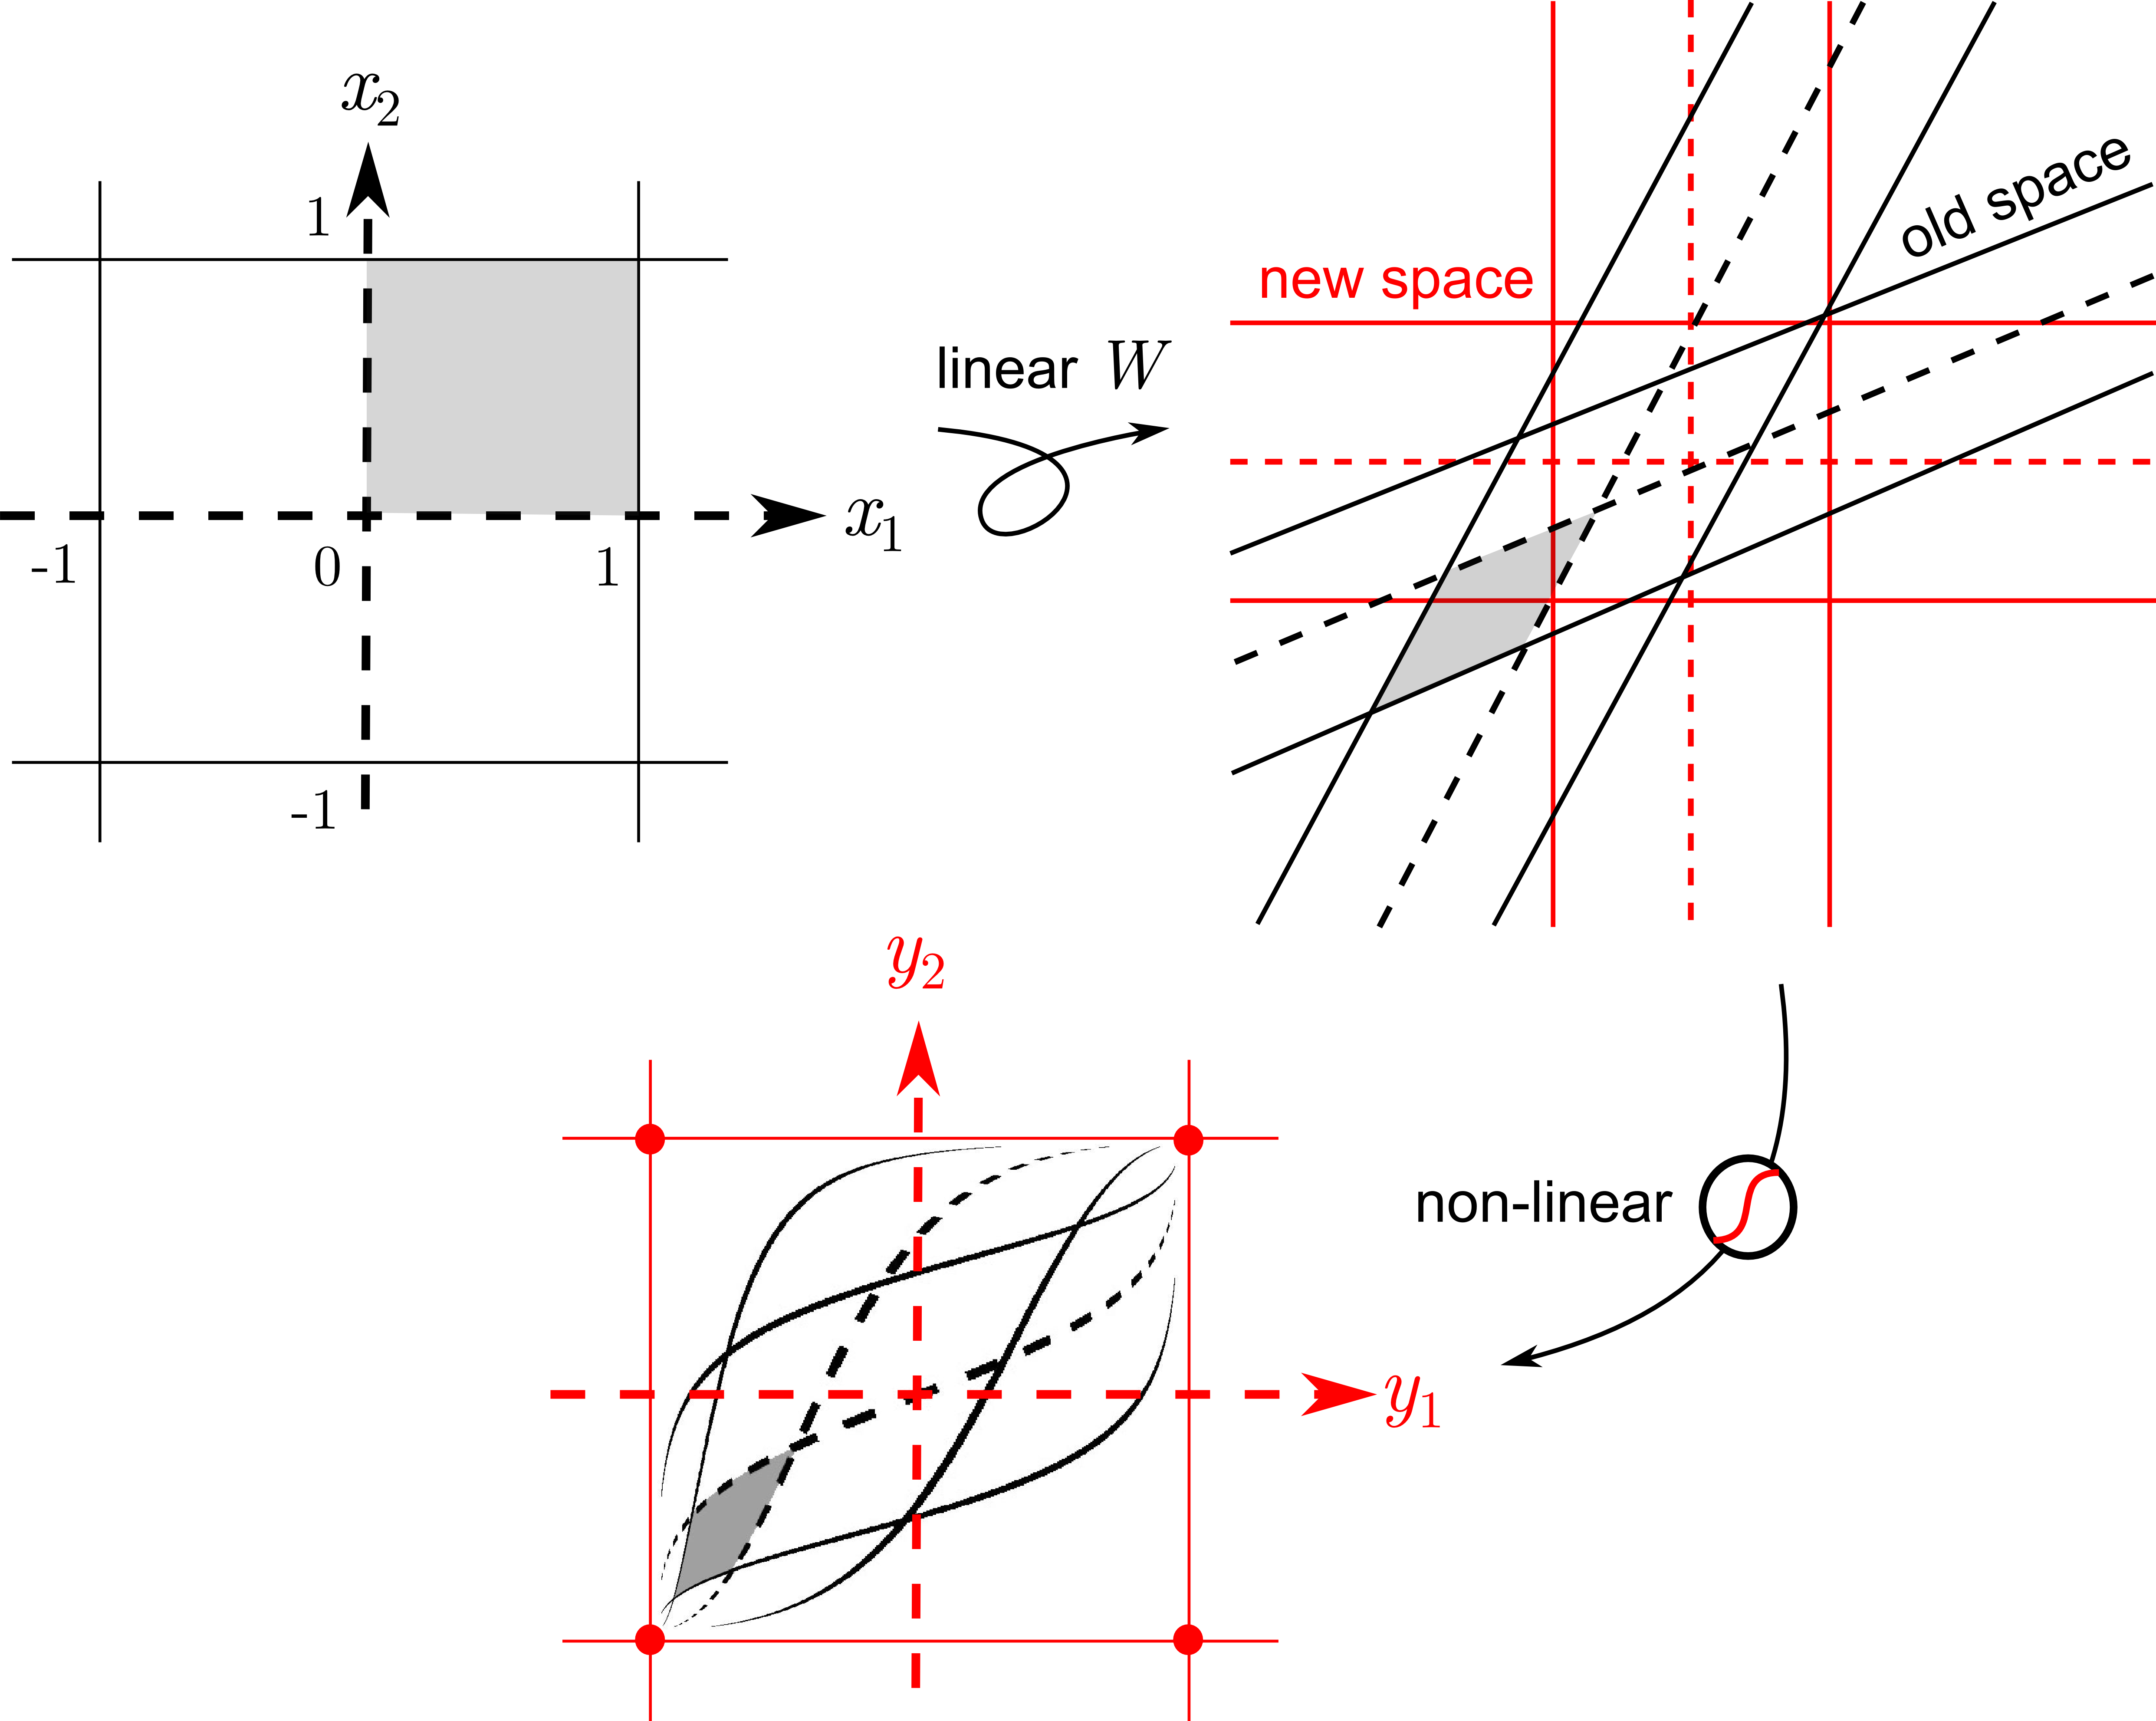
\includegraphics[scale=0.6]{NN-1-layer.png}}}
\end{equation}

%为简化讨论,现在只考虑 2 粒神经元的\textbf{输入}和\textbf{输出}空间(都是 2 度空间的平面):
%\begin{equation}
%\vcenter{\hbox{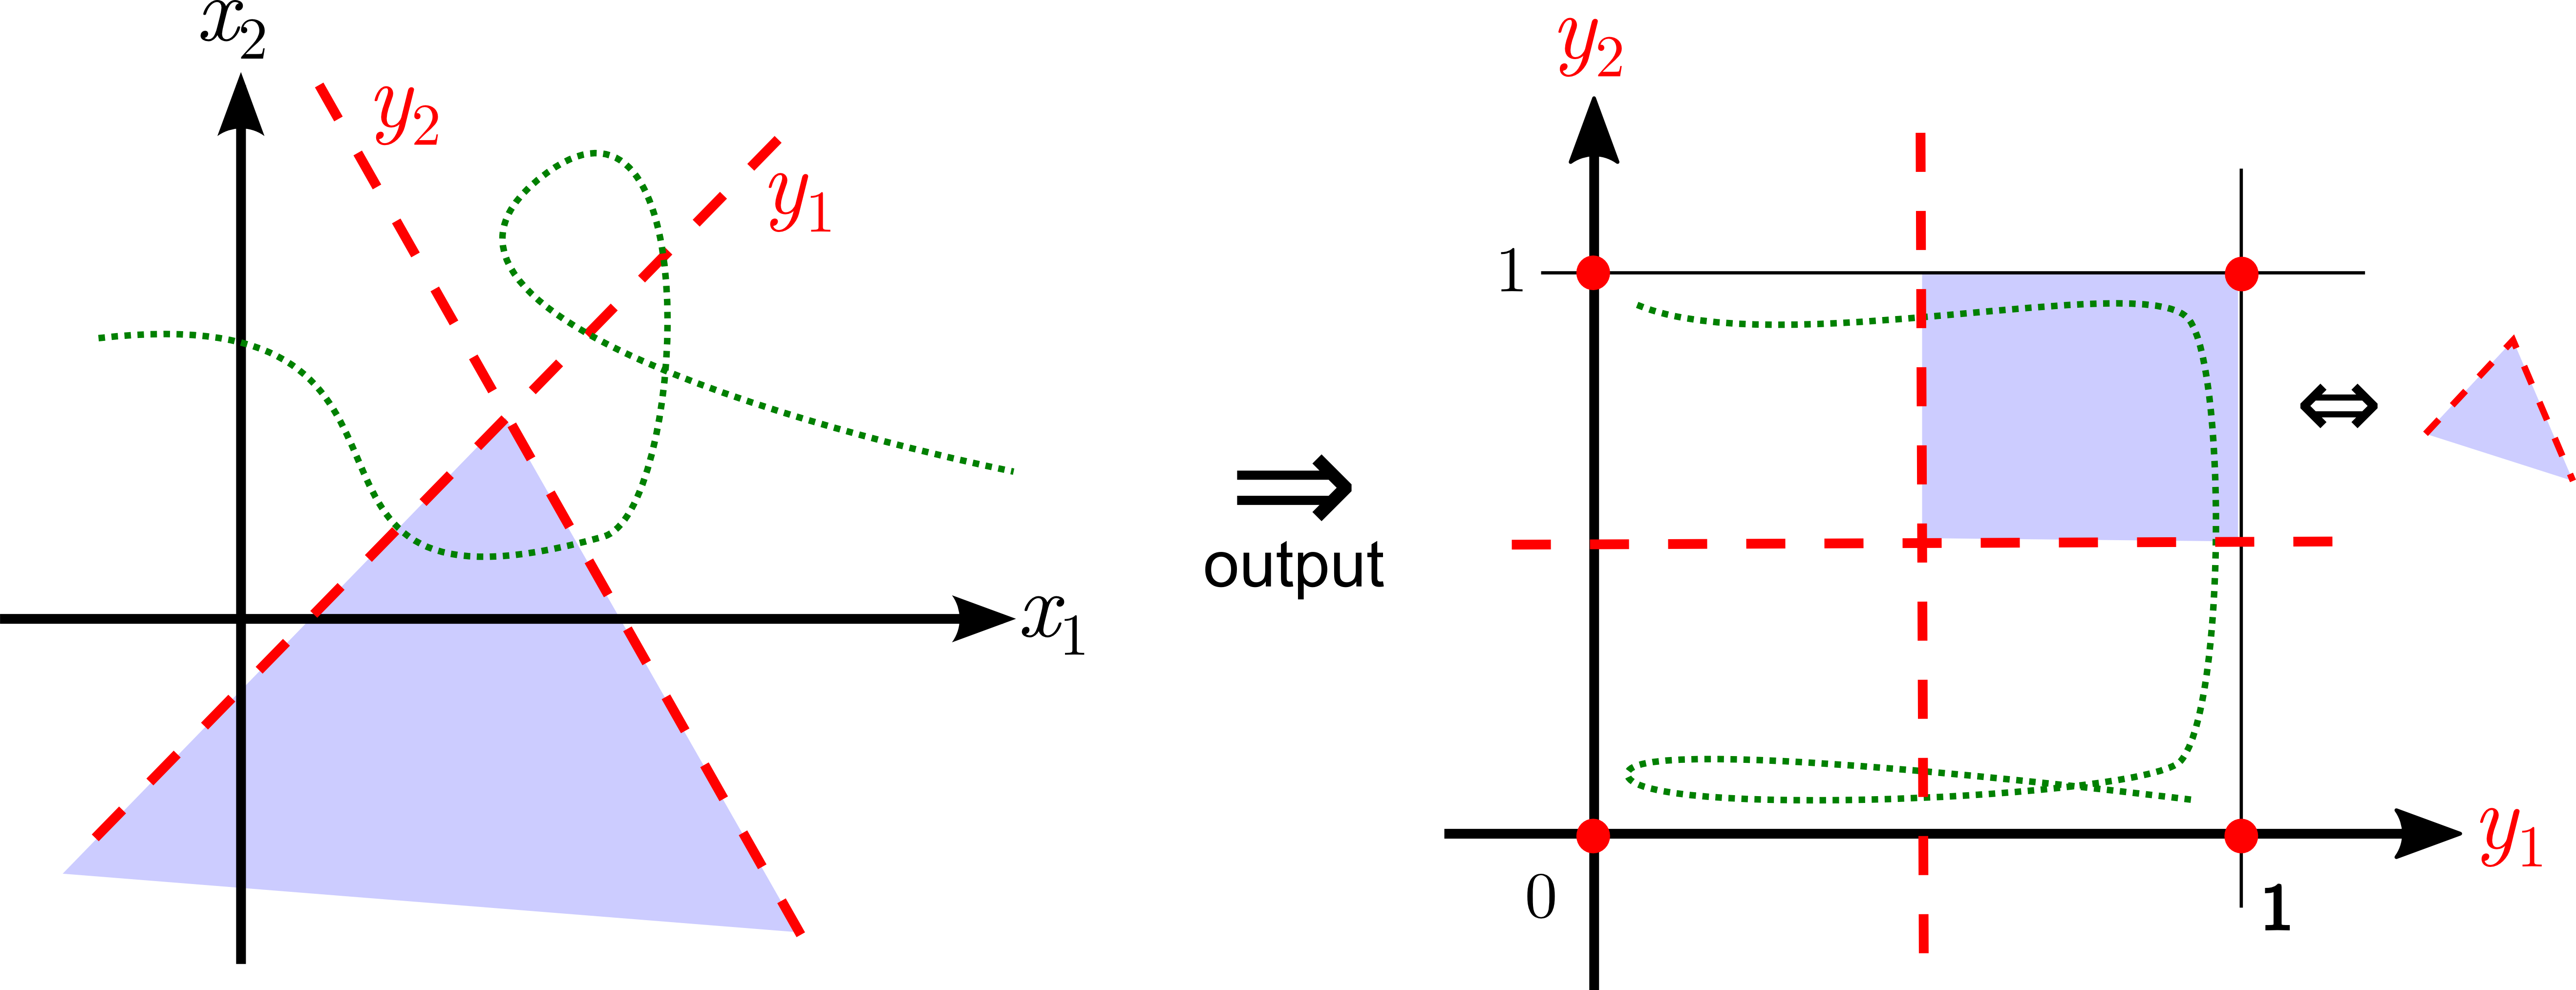
\includegraphics[scale=0.6]{linear-inequalities-3.png}}}
%\end{equation}
%因为 $\sigmoid$ 的缘故,输出的位置会趋近 hyper-cube 的那些 \textbf{顶点} ({\color{red}{\textbullet}})。 这些顶点对应於输入空间中被割开的 regions。 例如 {\color{cerulean}{蓝色}}那块 region 对应於:
%\begin{equation}
%(y_1 = \mbox{yes}, y_2 = \mbox{yes}) \quad \Rightarrow \quad (1,1)
%\end{equation}
%当输入位置随{\color{darkgreen}{绿色}}线游荡时,输出会在 hyper-cube 的顶点之间跳来跳去。 妳可能觉得这样移动很无聊(因为顶点个数不多),但当神经元的个数 $n$ 增加时,hyper-cube 的顶点个数会以 $2^n$ 的速度增长。 

\section*{Multi-layer neural network}

This is simply the repetition of single layers:
\begin{equation}
\boxed{output} \; \vect{y} = \sigmoid \stackrel{1}{W} \; \sigmoid \stackrel{2}{W} \; ..... \; \sigmoid \stackrel{L}{W} \; \vect{x}
\end{equation}
$L$ = total number of layers.

\centering{ --- The end --- }

% \href{http://genifer.googlecode.com/files/Genifer - induction (30 July 2012).pdf}{inductive learning (PDF, in English)}

%\bibliographystyle{plain} % or number or aaai ...
%\bibliography{AGI-book}

\end{document}
